\chapter{Results}
\label{c:result}

\section{Datasets}
\label{s:dataset}

%
% GSE52194 Breast cancer
% GSE52778 Airway Muscle and Asthma
%

Two RNA-Seq datasets and one DNA-Seq datasets from Gene Expression Omnibus
(GEO) were used for the demonstration of BioCloud. GSE52194
\cite{eswaran2012:transcriptomic} was a transcriptome profiling dataset of
human breast cancer. mRNA profiles of 17 breast tumor samples of three
different subtypes (TNBC, non-TNBC and HER2-positive) and normal human breast
organoids (epithelium) samples (NBS) were sequenced using Illumina HiSeq 2000
sequencer. Full sample list can be found in Table~\ref{tab:dataset-breast}.
Raw sequence reads were obtained from NCBI Sequence Read Archive (SRA), thus
their FASTQ file names were based on their SRA accession ID. In GSE52194 breast
cancer dataset, condition was defined to be the cancer subtype of the sample.

\begin{table}[!htbp]
    \caption[Experiment design of breast cancer GSE52194]{
        Experiment design of breast cancer dataset GSE52194.
    }
    \label{tab:dataset-breast}
    \centering
    \begin{threeparttable}
        \begin{tabular}{llr}
            \toprule
            Condition & Sample name & SRA ID and filename \\
            \midrule
            NBS      & NBS1      & SRR1027188 \\
            NBS      & NBS2      & SRR1027189 \\
            NBS      & NBS3      & SRR1027190 \\
            TNBC     & TNBC1     & SRR1027171 \\
            TNBC     & TNBC2     & SRR1027172 \\
            TNBC     & TNBC3     & SRR1027173 \\
            TNBC     & TNBC4     & SRR1027174 \\
            TNBC     & TNBC5     & SRR1027175 \\
            TNBC     & TNBC6     & SRR1027176 \\
            Non-TNBC & Non-TNBC1 & SRR1027177 \\
            Non-TNBC & Non-TNBC2 & SRR1027178 \\
            Non-TNBC & Non-TNBC3 & SRR1027179 \\
            Non-TNBC & Non-TNBC4 & SRR1027180 \\
            Non-TNBC & Non-TNBC5 & SRR1027181 \\
            Non-TNBC & Non-TNBC6 & SRR1027182 \\
            HER2     & HER2-1    & SRR1027183 \\
            HER2     & HER2-2    & SRR1027184 \\
            HER2     & HER2-3    & SRR1027185 \\
            HER2     & HER2-4    & SRR1027186 \\
            HER2     & HER2-5    & SRR1027187 \\
            \bottomrule
        \end{tabular}
    \end{threeparttable}
\end{table}


Another RNA-Seq dataset, GSE52778 \cite{himes2014:rnaseq}, is a transcriptome
profiling dataset of human airway smooth muscle (HASM). mRNA profiles of 4 male
white donors' HASM cells treated with four treatment conditions were sequenced
using Illumina HiSeq 2000 sequencer with Illumina TruSeq assay, four treatment
conditions being: no treatment (Untreated); treatment with Albuterol (Alb);
treatment with Dexamethasone (Dex); treatment with simultaneous Albuterol and
Dexamethasone (Alb\_Dex). Full sample list can be found in
Table~\ref{tab:dataset-airway}. Raw sequence reads were obtained from SRA thus
sample raw FASTQ files are renamed using their SRA accession ID.

\begin{table}[!htbp]
    \caption[Experiment design of GSE52778 airway muscle dataset]{
        Experiment design of GSE52778 airway muscle dataset.
    }
    \label{tab:dataset-airway}
    \centering
    \begin{threeparttable}
        \begin{tabular}{llr}
            \toprule
            Condition & Sample name & SRA Accession ID \\
            \midrule
            Untreated & N61311\_Untreated  & SRR1039508 \\
            Untreated & N052611\_Untreated & SRR1039512 \\
            Untreated & N080611\_Untreated & SRR1039516 \\
            Untreated & N061011\_Untreated & SRR1039520 \\

            Dex       & N61311\_Dex        & SRR1039509 \\
            Dex       & N052611\_Dex       & SRR1039513 \\
            Dex       & N080611\_Dex       & SRR1039517 \\
            Dex       & N061011\_Dex       & SRR1039521 \\

            Alb       & N61311\_Alb        & SRR1039510 \\
            Alb       & N052611\_Alb       & SRR1039514 \\
            Alb       & N080611\_Alb       & SRR1039518 \\
            Alb       & N061011\_Alb       & SRR1039522 \\

            Alb\_Dex  & N61311\_Alb\_Dex   & SRR1039511 \\
            Alb\_Dex  & N052611\_Alb\_Dex\tnote{$\dagger$} & SRR1039515\tnote{$\dagger$} \\
            Alb\_Dex  & N080611\_Alb\_Dex  & SRR1039519 \\
            Alb\_Dex  & N061011\_Alb\_Dex  & SRR1039523 \\
            \bottomrule
        \end{tabular}
        \begin{tablenotes}
        \item[$\dagger$] This sample was excluded from the later-on analyses
            since its pair-end sequencing reads were mismatched.
        \end{tablenotes}
    \end{threeparttable}
\end{table}


% TODO: how deep is the sequencing depth of these WES samples?

The DNA-Seq dataset used in the demonstration was a human whole exome
sequencing done in our lab. Exome sequencing of 5 members from the same family
using Illumina HiSeq 2000 sequencer. The study aimed to find the common
variants shared in this family.



\section{Account registration and user dashboard}

A new user account was registered on BioCloud using email
\texttt{demo@biocloud.liang2.io}. Screenshots of the registration process are
shown in Figure~\ref{fig:biocloud-signup}, which resemble the process on common
websites. Most of the user inputs were sanity checked and validated, as shown
in Figure~\ref{fig:biocloud-signup}(b). After user completed the form, a
verification email was sent to the registered email address so as to make sure
all future email notifications can reach the user. A fixed message is displayed
on all pages of BioCloud if the user does not complete the email verification,
as shown in Figure~\ref{fig:biocloud-signup}(c).
Figure~\ref{fig:biocloud-signup}(d) shows the content of the verification
email, where an uniquely HMAC-based verification link was given. After clicking
on the link, user completed the verification and the fixed message for
verification was gone, as shown in Figure~\ref{fig:biocloud-signup}(e).

\begin{figure}[!p]
\centering
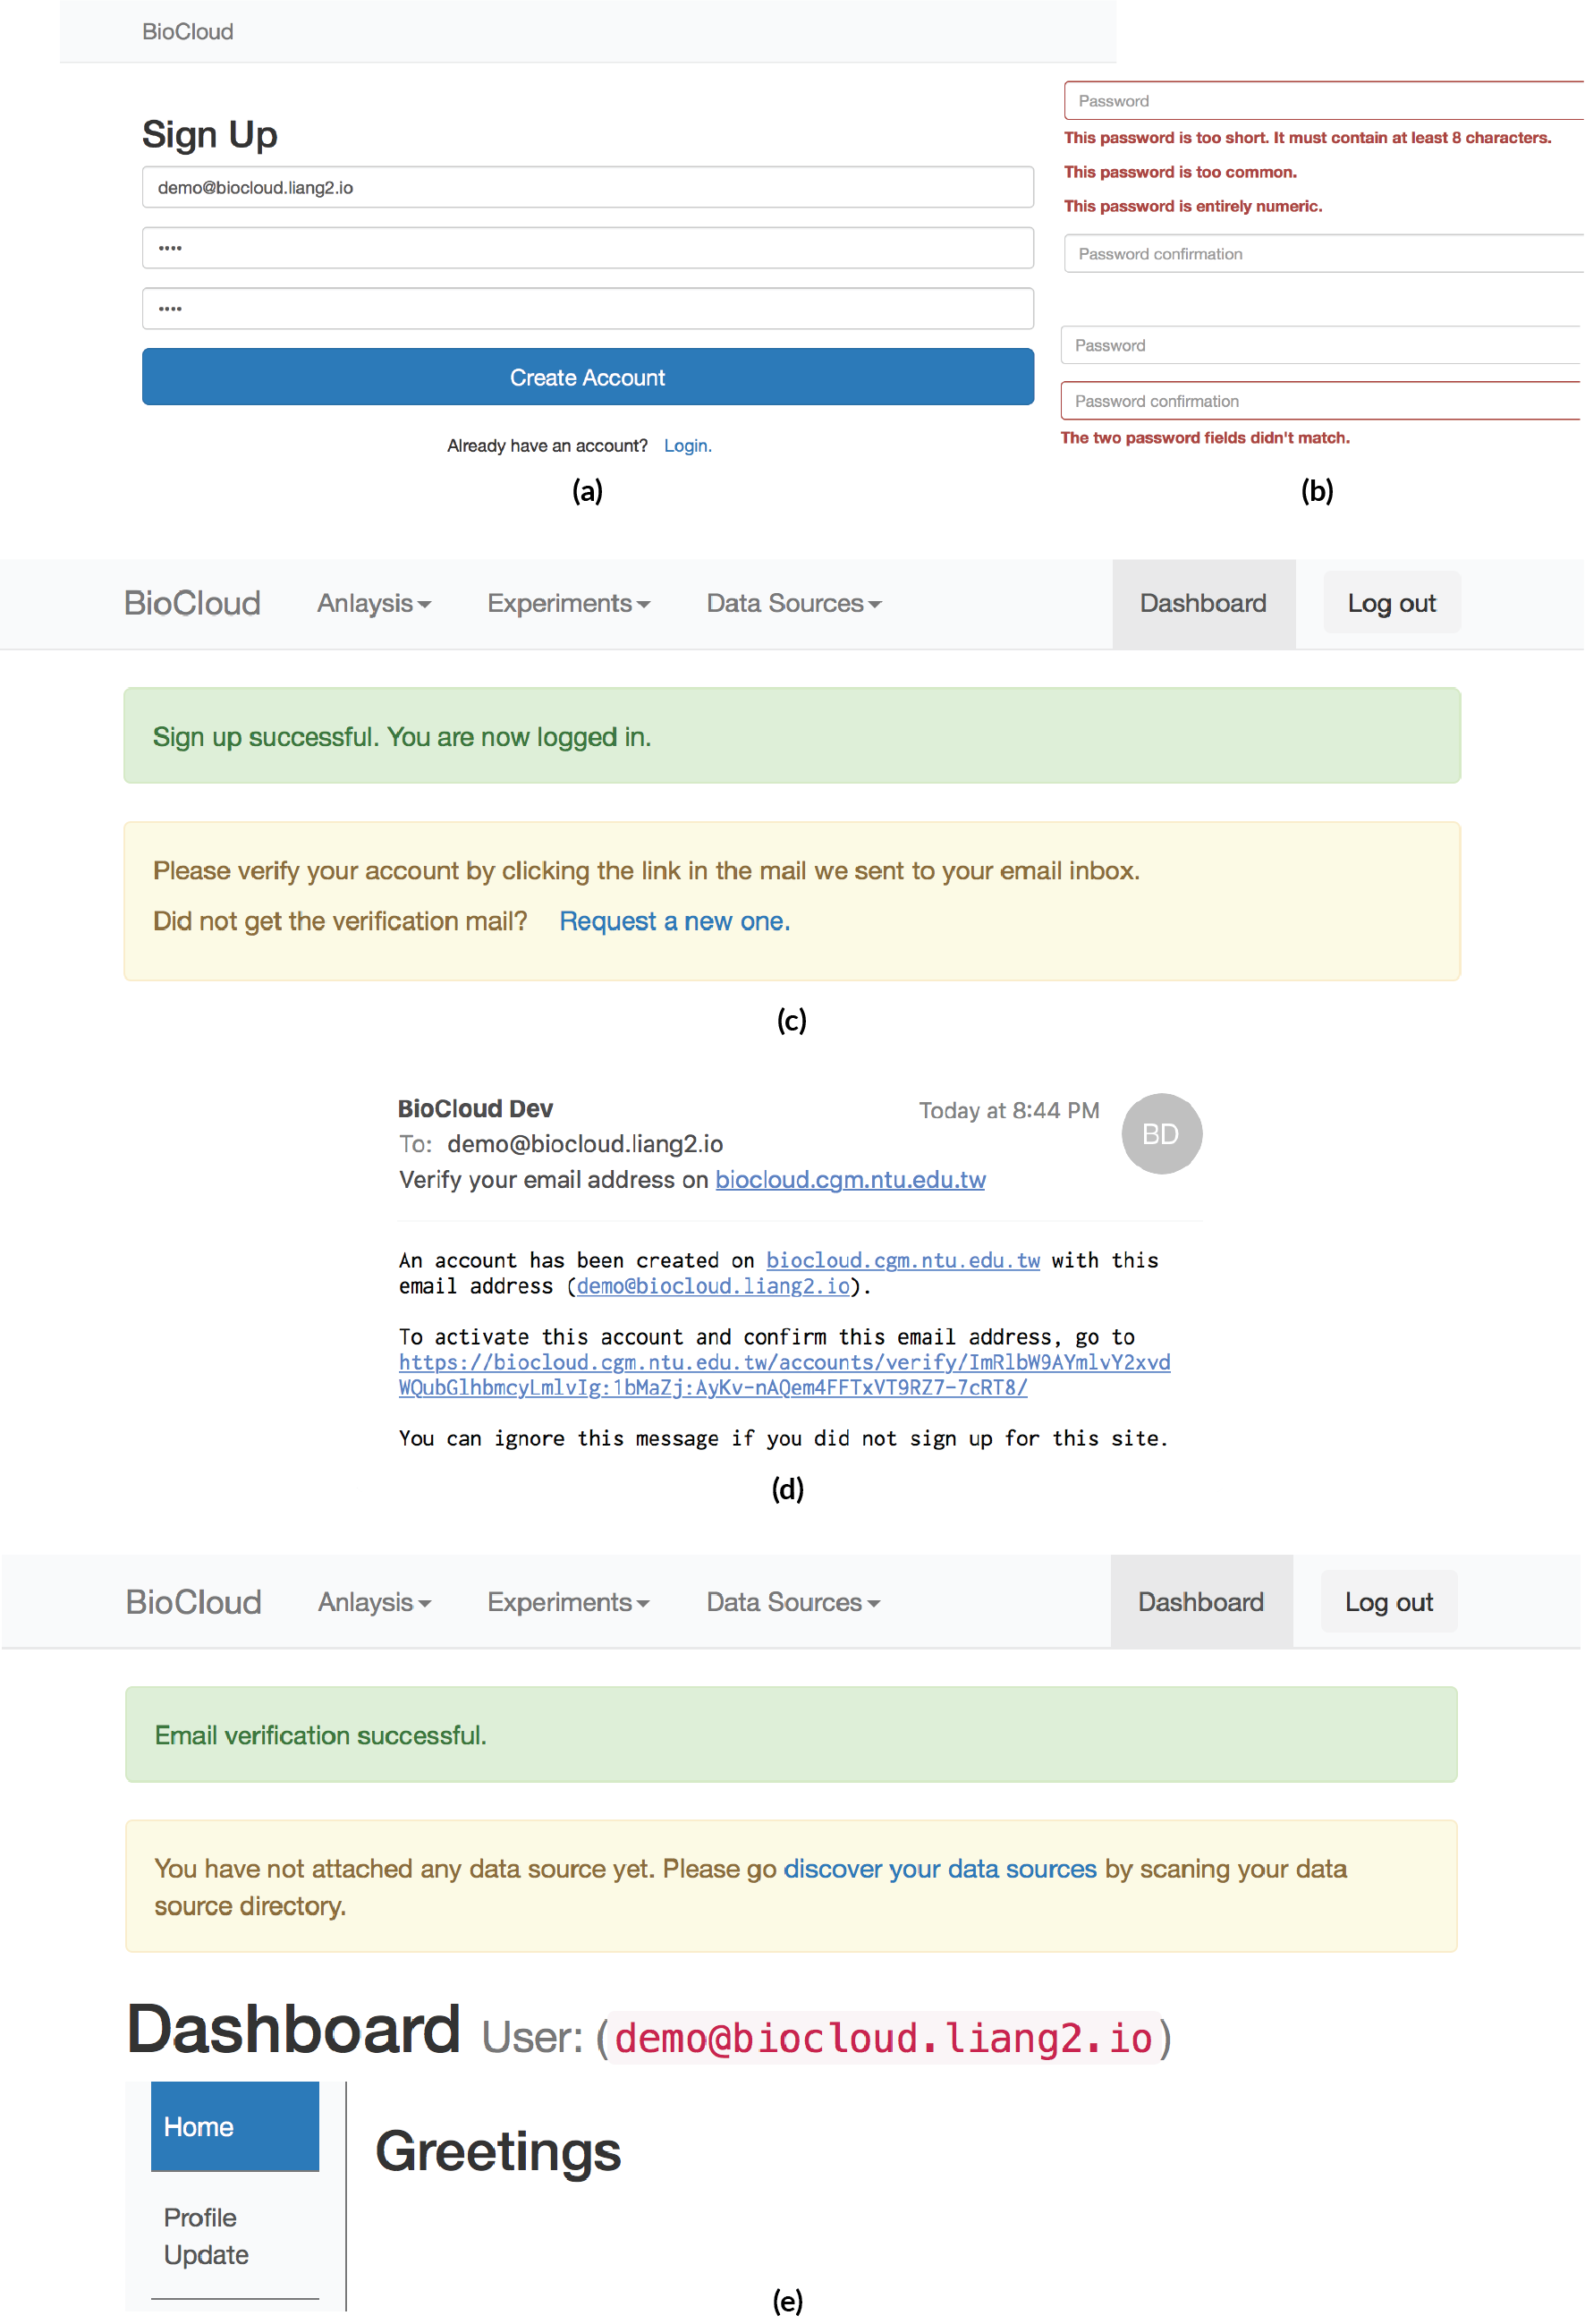
\includegraphics[width=1\textwidth]{images/biocloud_signup}
\caption[Account registration on BioCloud]{
    Account registration on BioCloud.
    (a) Registration form.
    (b) Password validation check.
    (c) Welcome screen after signup with action hint messages.
    (d) Verification email.
    (e) Welcome screen after email verifiction.
}
\label{fig:biocloud-signup}
\end{figure}


A user dashboard is available for user-related settings as shown in
Figure~\ref{fig:biocloud-dashboard}(b). User profile including user name and
authentication number (more on Section~\ref{s:report-result-access}) can be
updated here. Password can be changed via the link in the password section in
profile update, as shown in Figure~\ref{fig:biocloud-dashboard}(b). For staff
and superuser with special permission, they can access to the admin interface
of BioCloud in user dashboard via an extra tab ``Admin'', as shown in
Figure~\ref{fig:biocloud-dashboard}(d). Admin interface will be introduced in
Section~\ref{s:biocloud-admin}.

\begin{figure}[!p]
\centering
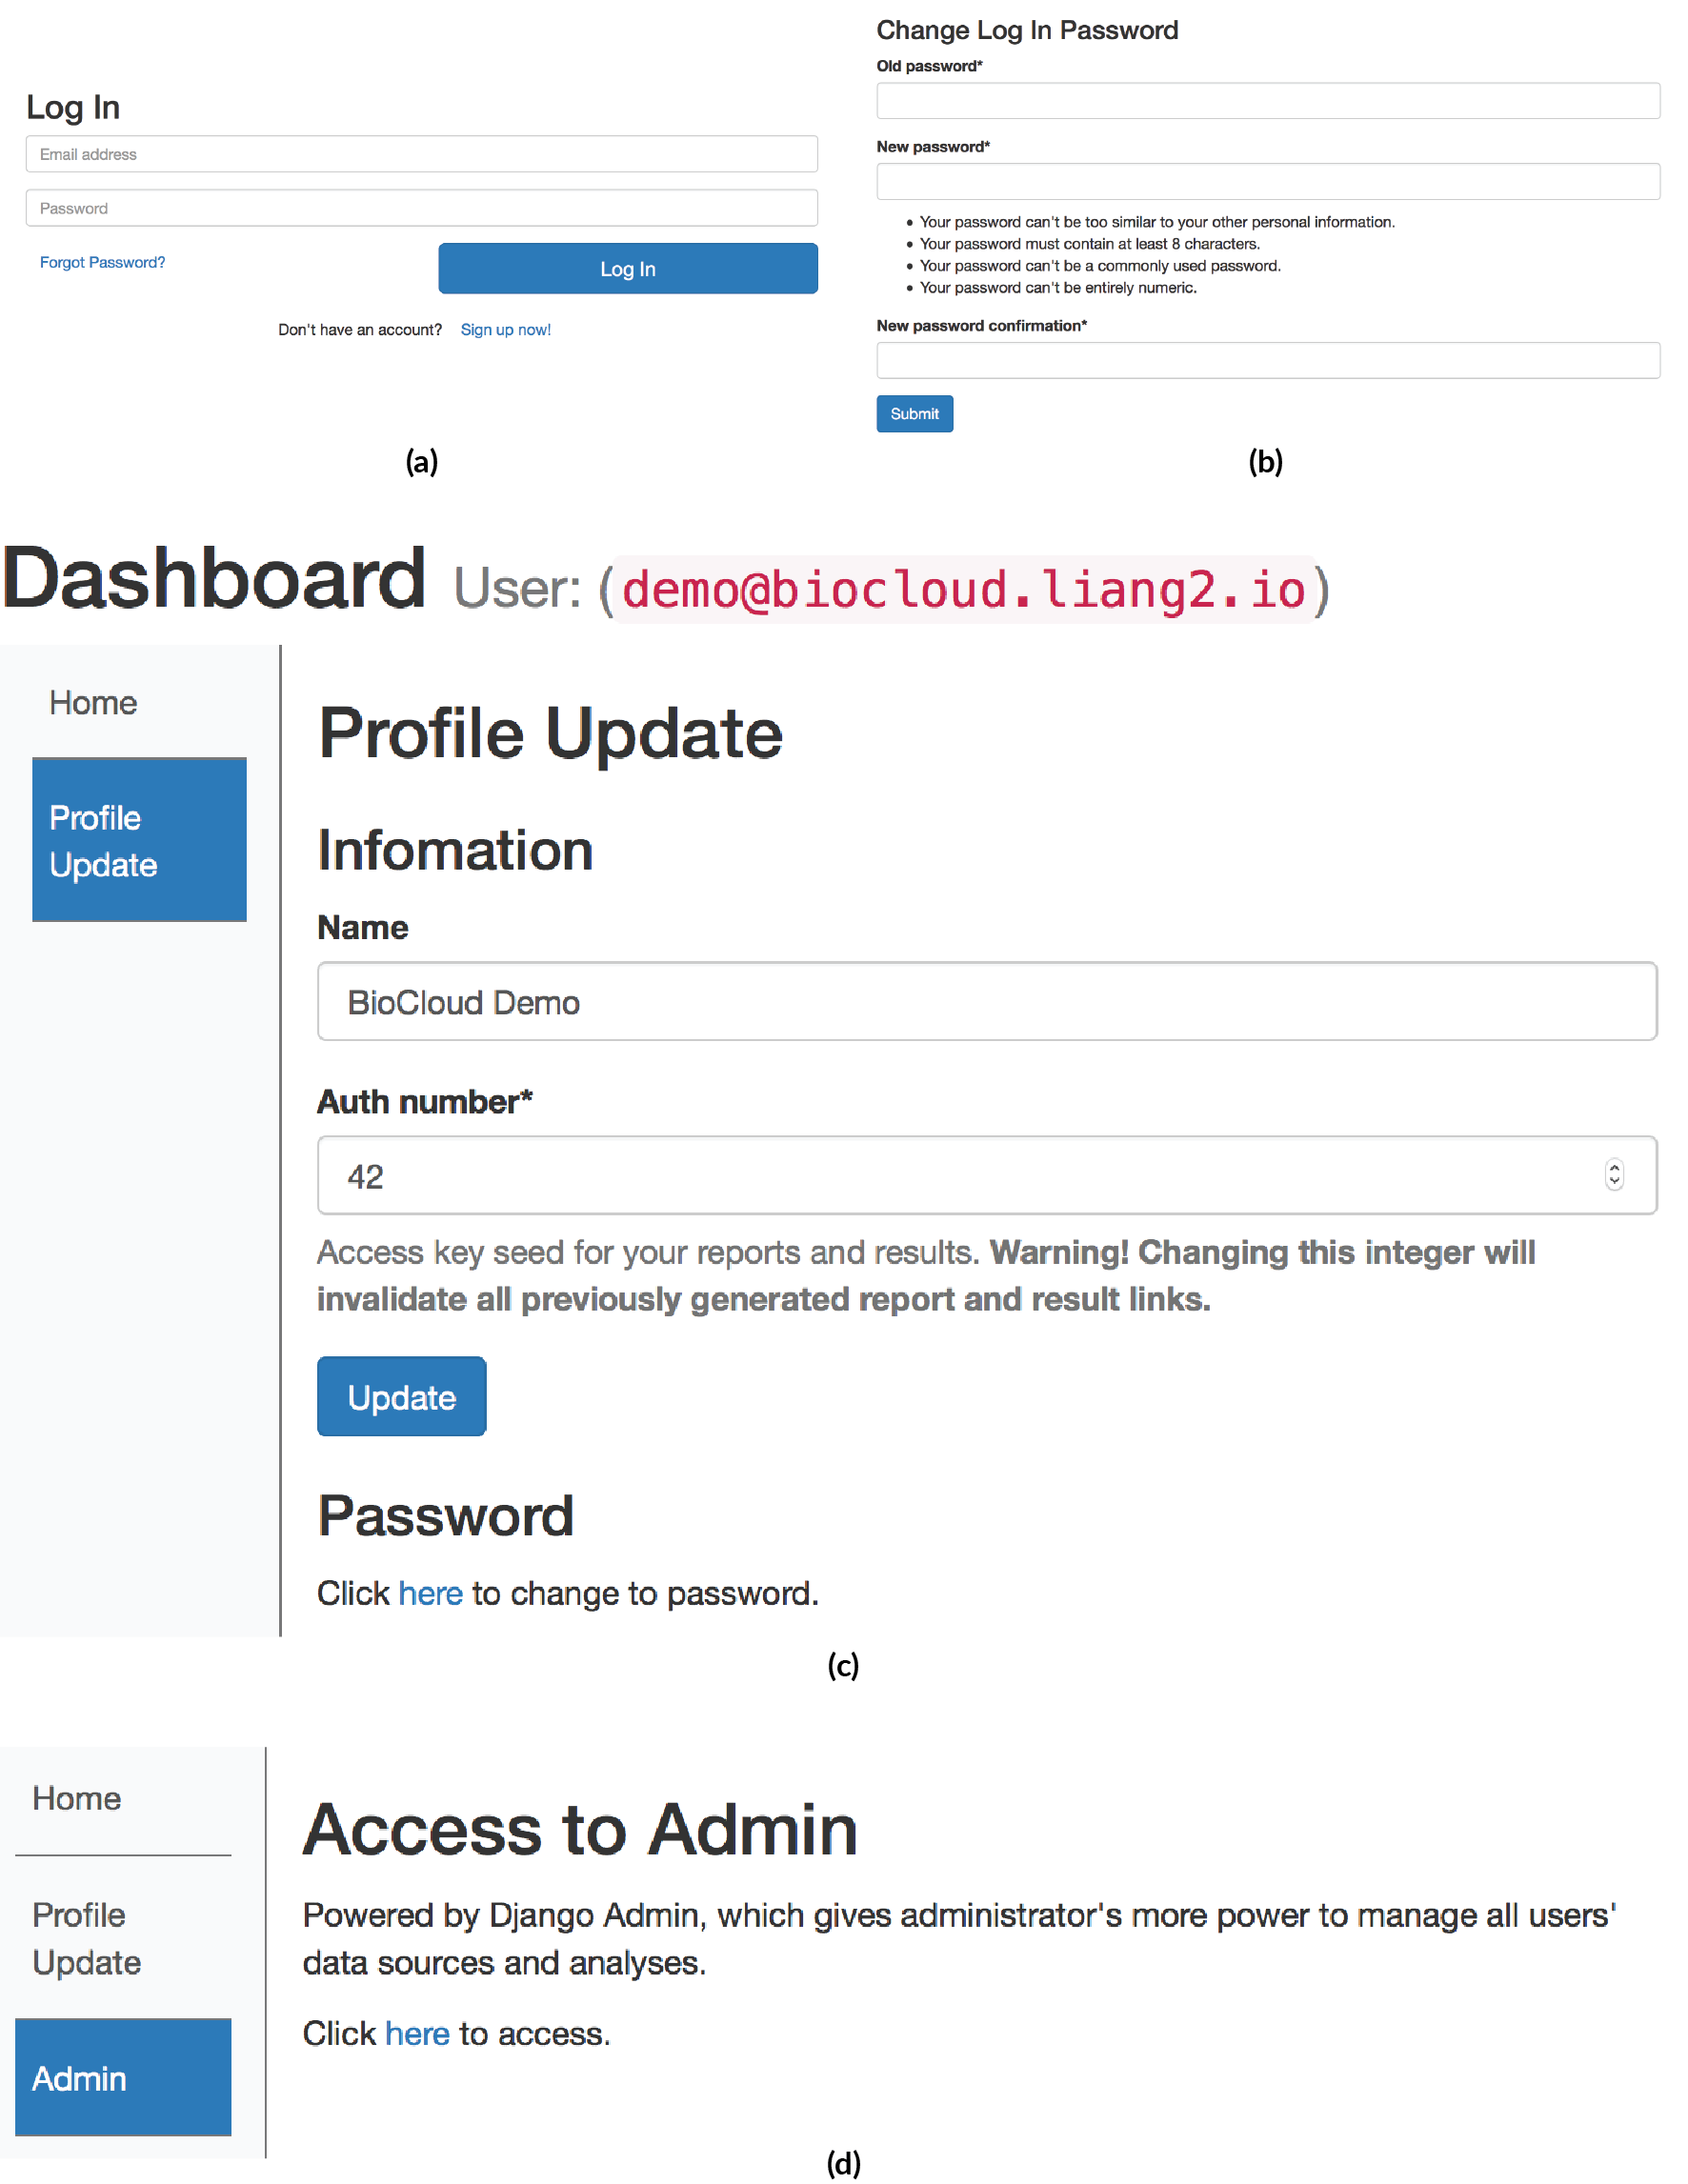
\includegraphics[width=1\textwidth]{images/biocloud_dashboard}
\caption[Login and user dashboard on BioCloud]{
    Login and user dashboard on BioCloud.
    (a) Login form.
    (b) Password change form available through profile update.
    (c) Profile update form.
    (d) For staff and superuser's dashboard, an extra tab to the admin
    interface is shown.
}
\label{fig:biocloud-dashboard}
\end{figure}





\section{Data source discovery}

As a newly registered user, a message was always shown to hint user to attach
their data sources to BioCloud. User can find their specific data source folder
from menu Data Source \textrightarrow List, as shown in
Figure~\ref{fig:biocloud-data-source}(b). For the demo user, location of the
data source folder on BioCloud server was:

\begin{CVerbatim}[fontsize=\small]
/biocloud/data_sources/2/
\end{CVerbatim}

\vspace{-1em}\noindent
Upon new data sources being added, BioCloud updated its database by comparing
the data sources in record with that in current folder. All new discovered data
sources will be listed with guess of sample name and file type, as shown in
Figure~\ref{fig:biocloud-data-source}(a). User can pass the SHA2-256 checksum
value for each file computed locally. BioCloud computed the checksum of these
files and compared the value with that supplied by the user. User can check and
update the detail of their recorded data sources, as shown in
Figure~\ref{fig:biocloud-data-source}(b). BioCloud also guessed the strand for
pair-end FASTA/Q files. The information was recorded at the metadata column in
JSON format.

\begin{figure}[!tbp]
\centering
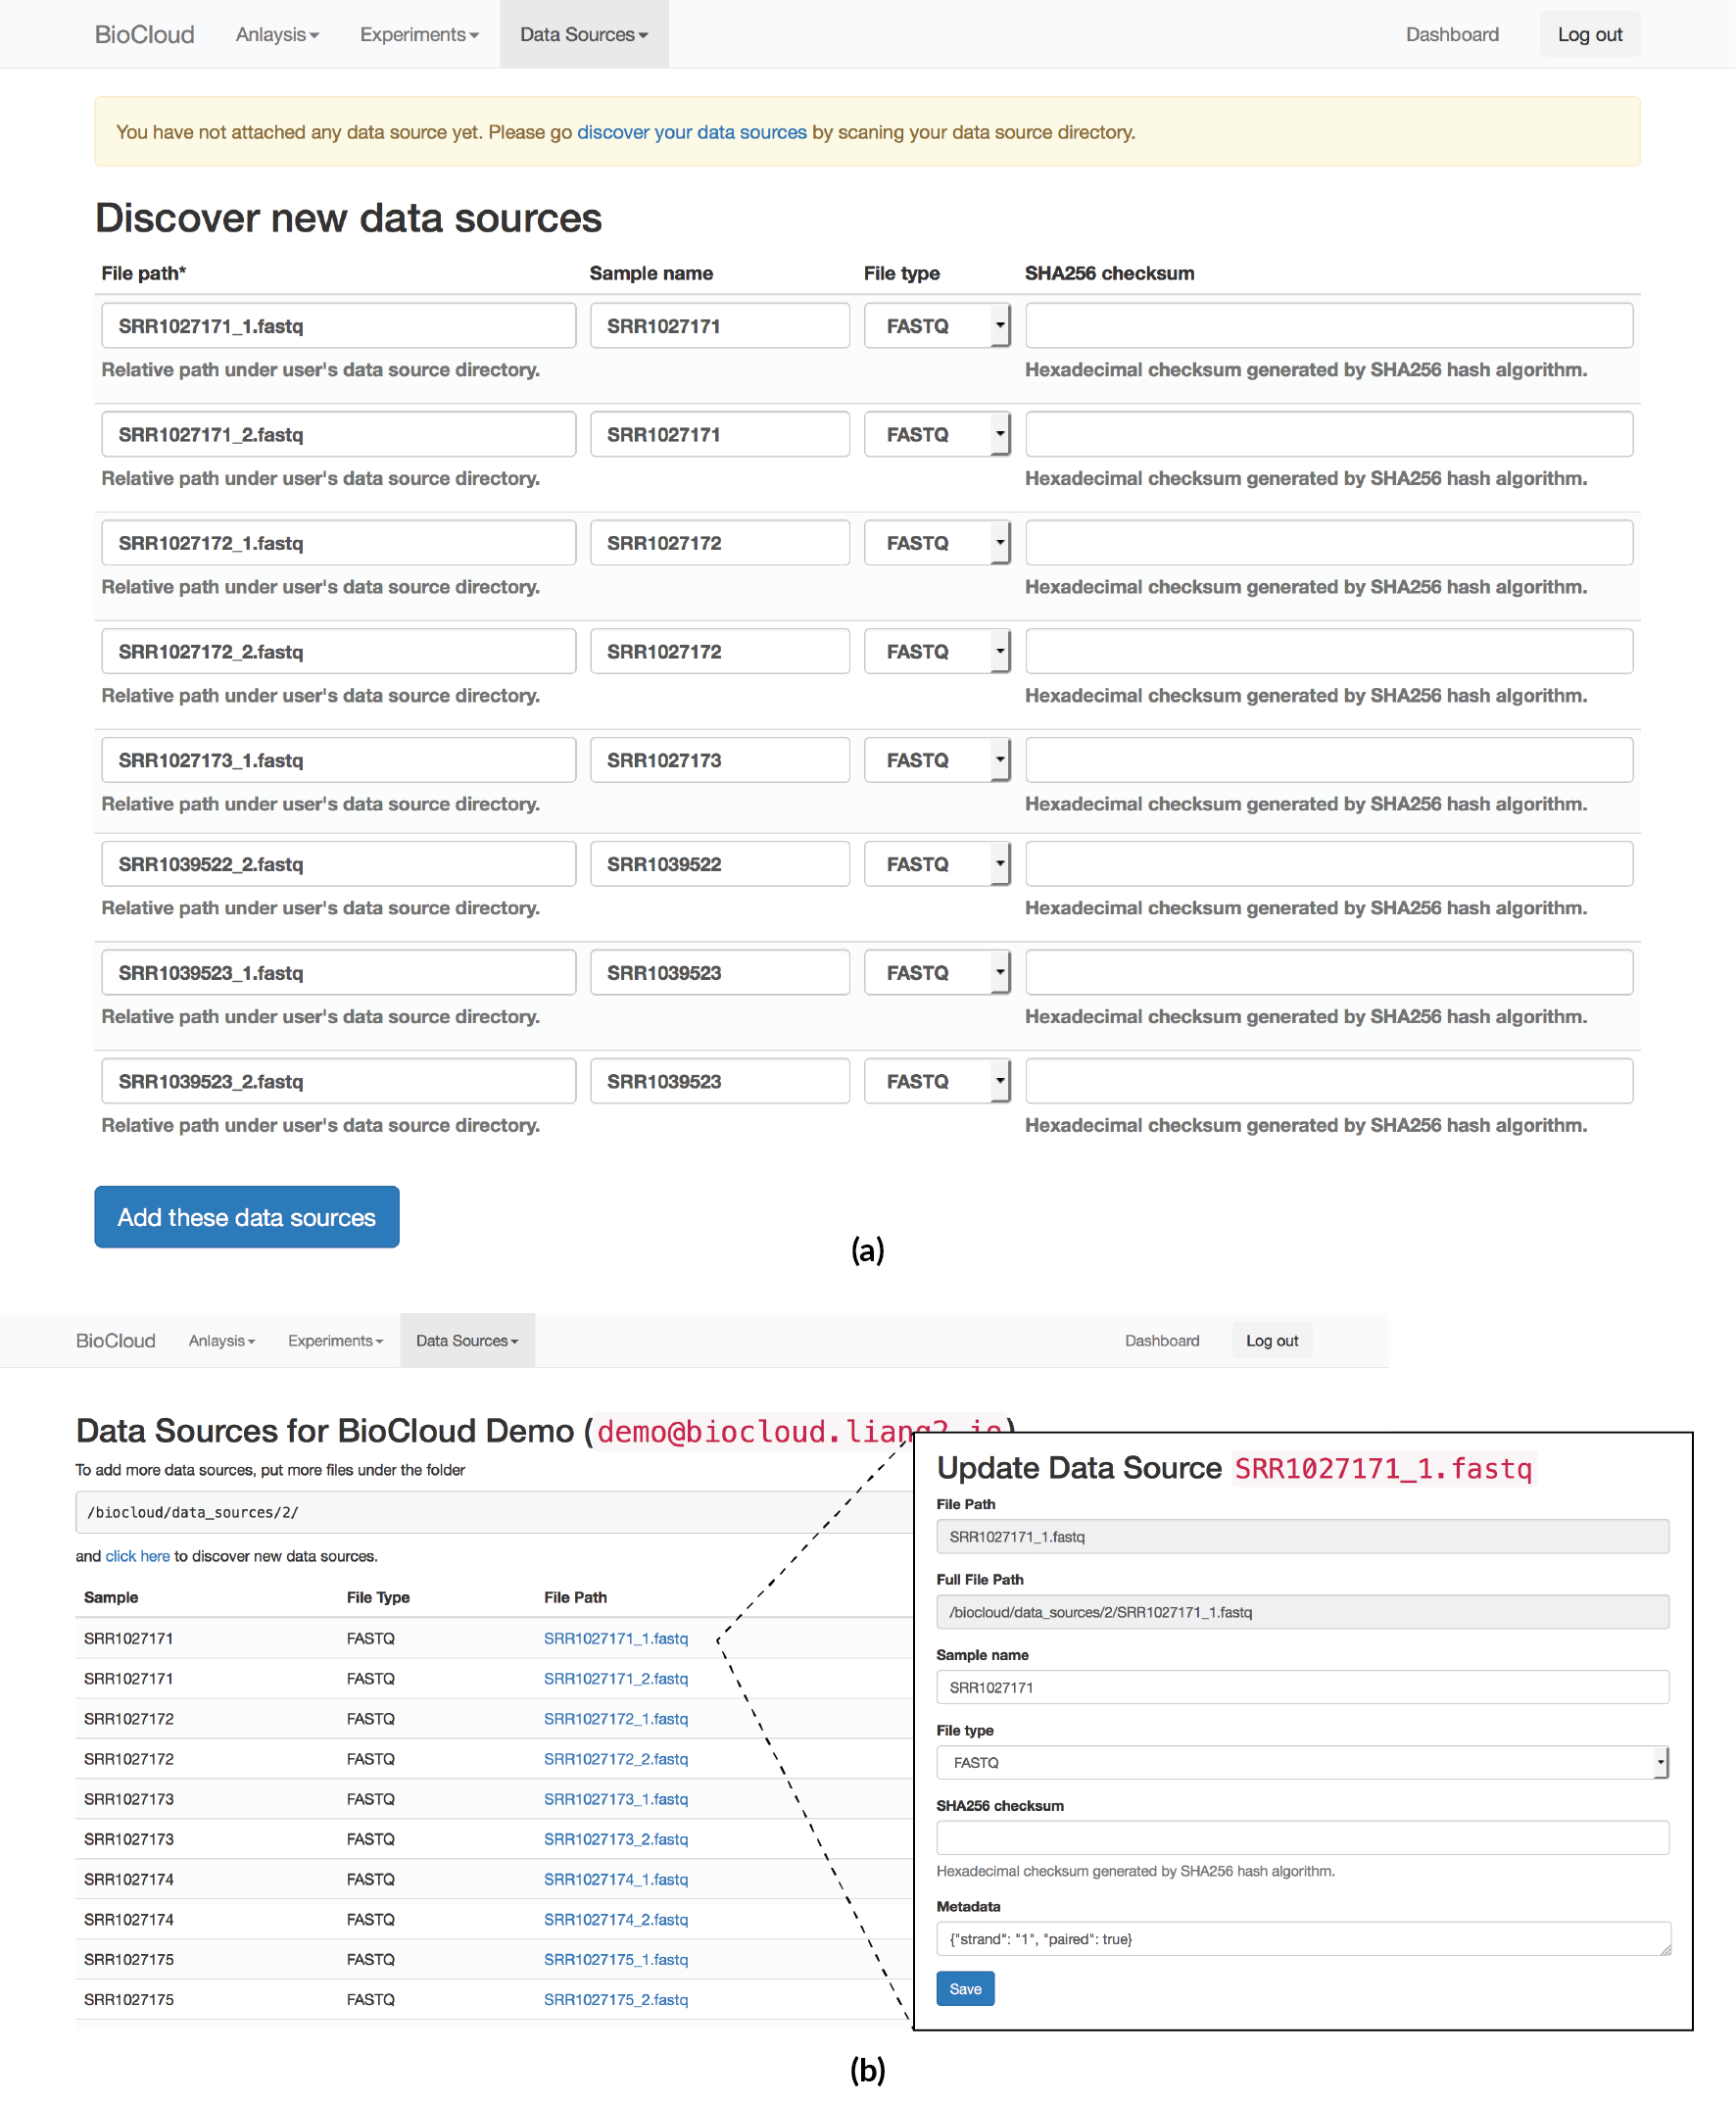
\includegraphics[width=1\textwidth]{images/biocloud_data_source}
\caption[Data source management on BioCloud]{
    Data source management on BioCloud.
    (a) Discovery of new ata sources.
    (b) List and detail view of data sources.
}
\label{fig:biocloud-data-source}
\end{figure}





\section{Experiment design}

\begin{figure}[!tbp]
\centering
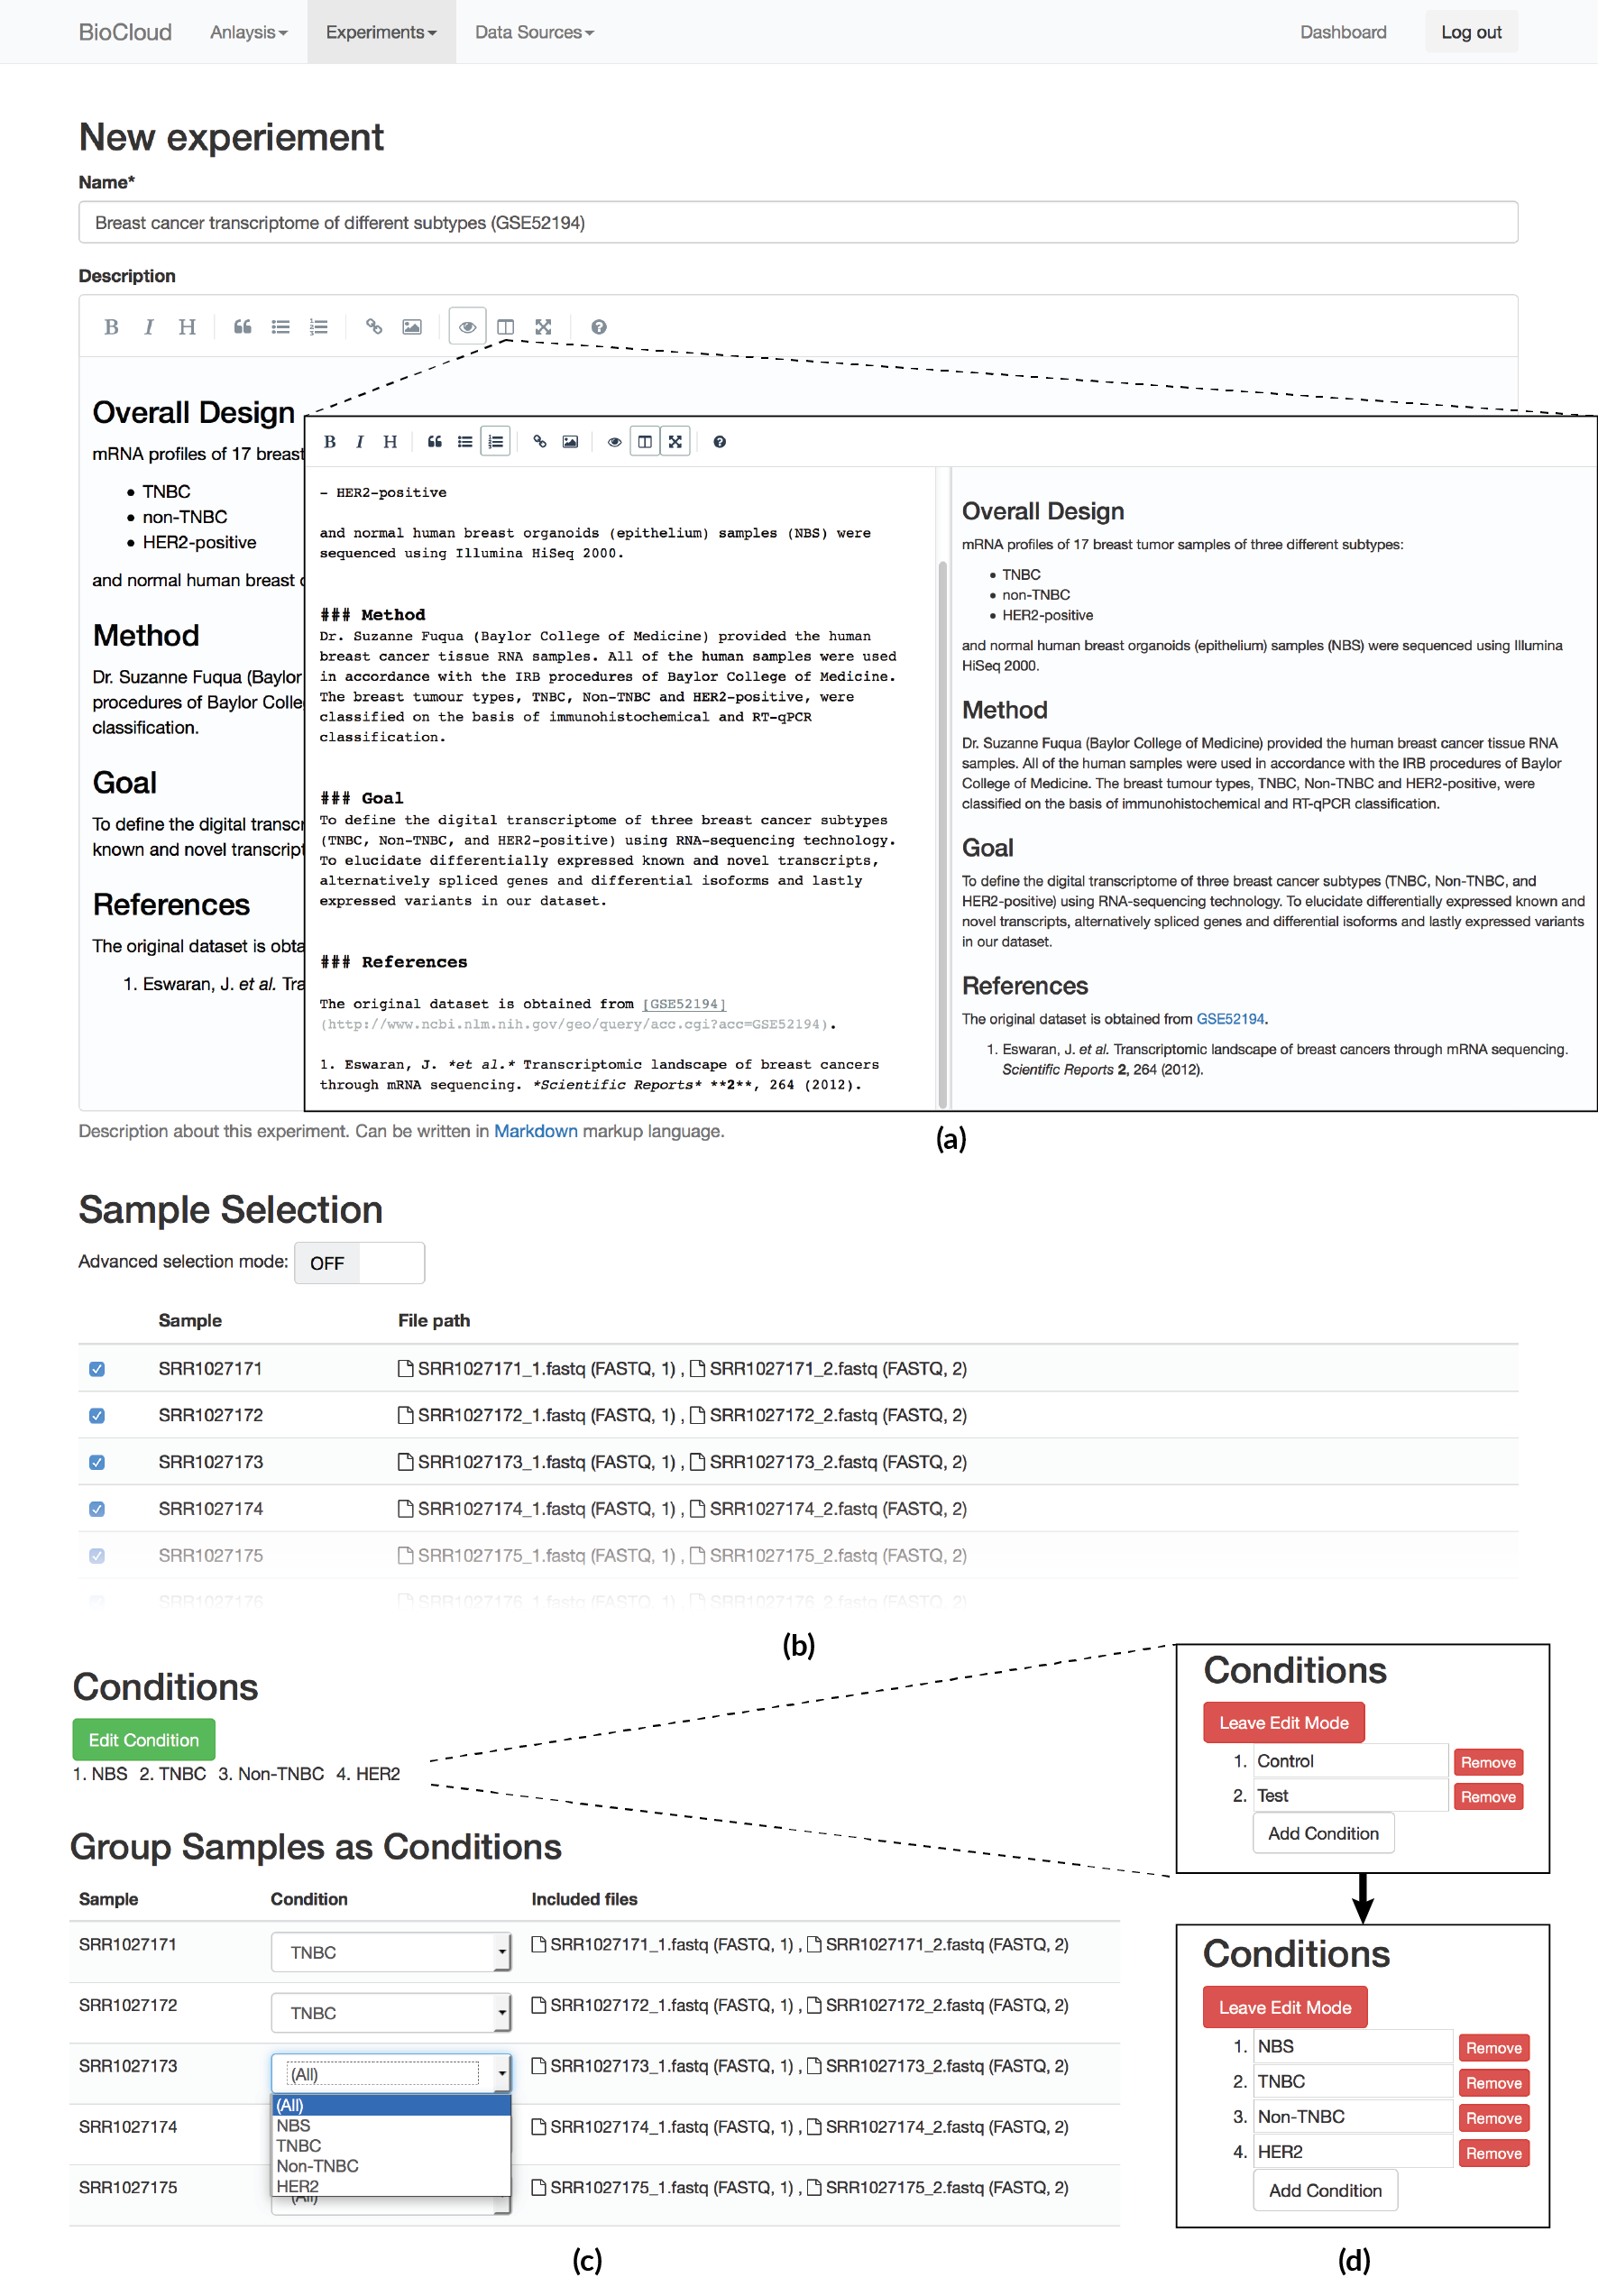
\includegraphics[width=1\textwidth]{images/biocloud_experiment_design}
\caption[Experiment design on BioCloud]{
    Experiment design on BioCloud.
    (a) Description Markdown editor in full screen.
    (b) Upper half of the experiment design form.
    (c) Condition assignment of samples.
    (d) Condition design.
}
\label{fig:biocloud-experiment-design}
\end{figure}

\begin{figure}[!tbp]
\centering
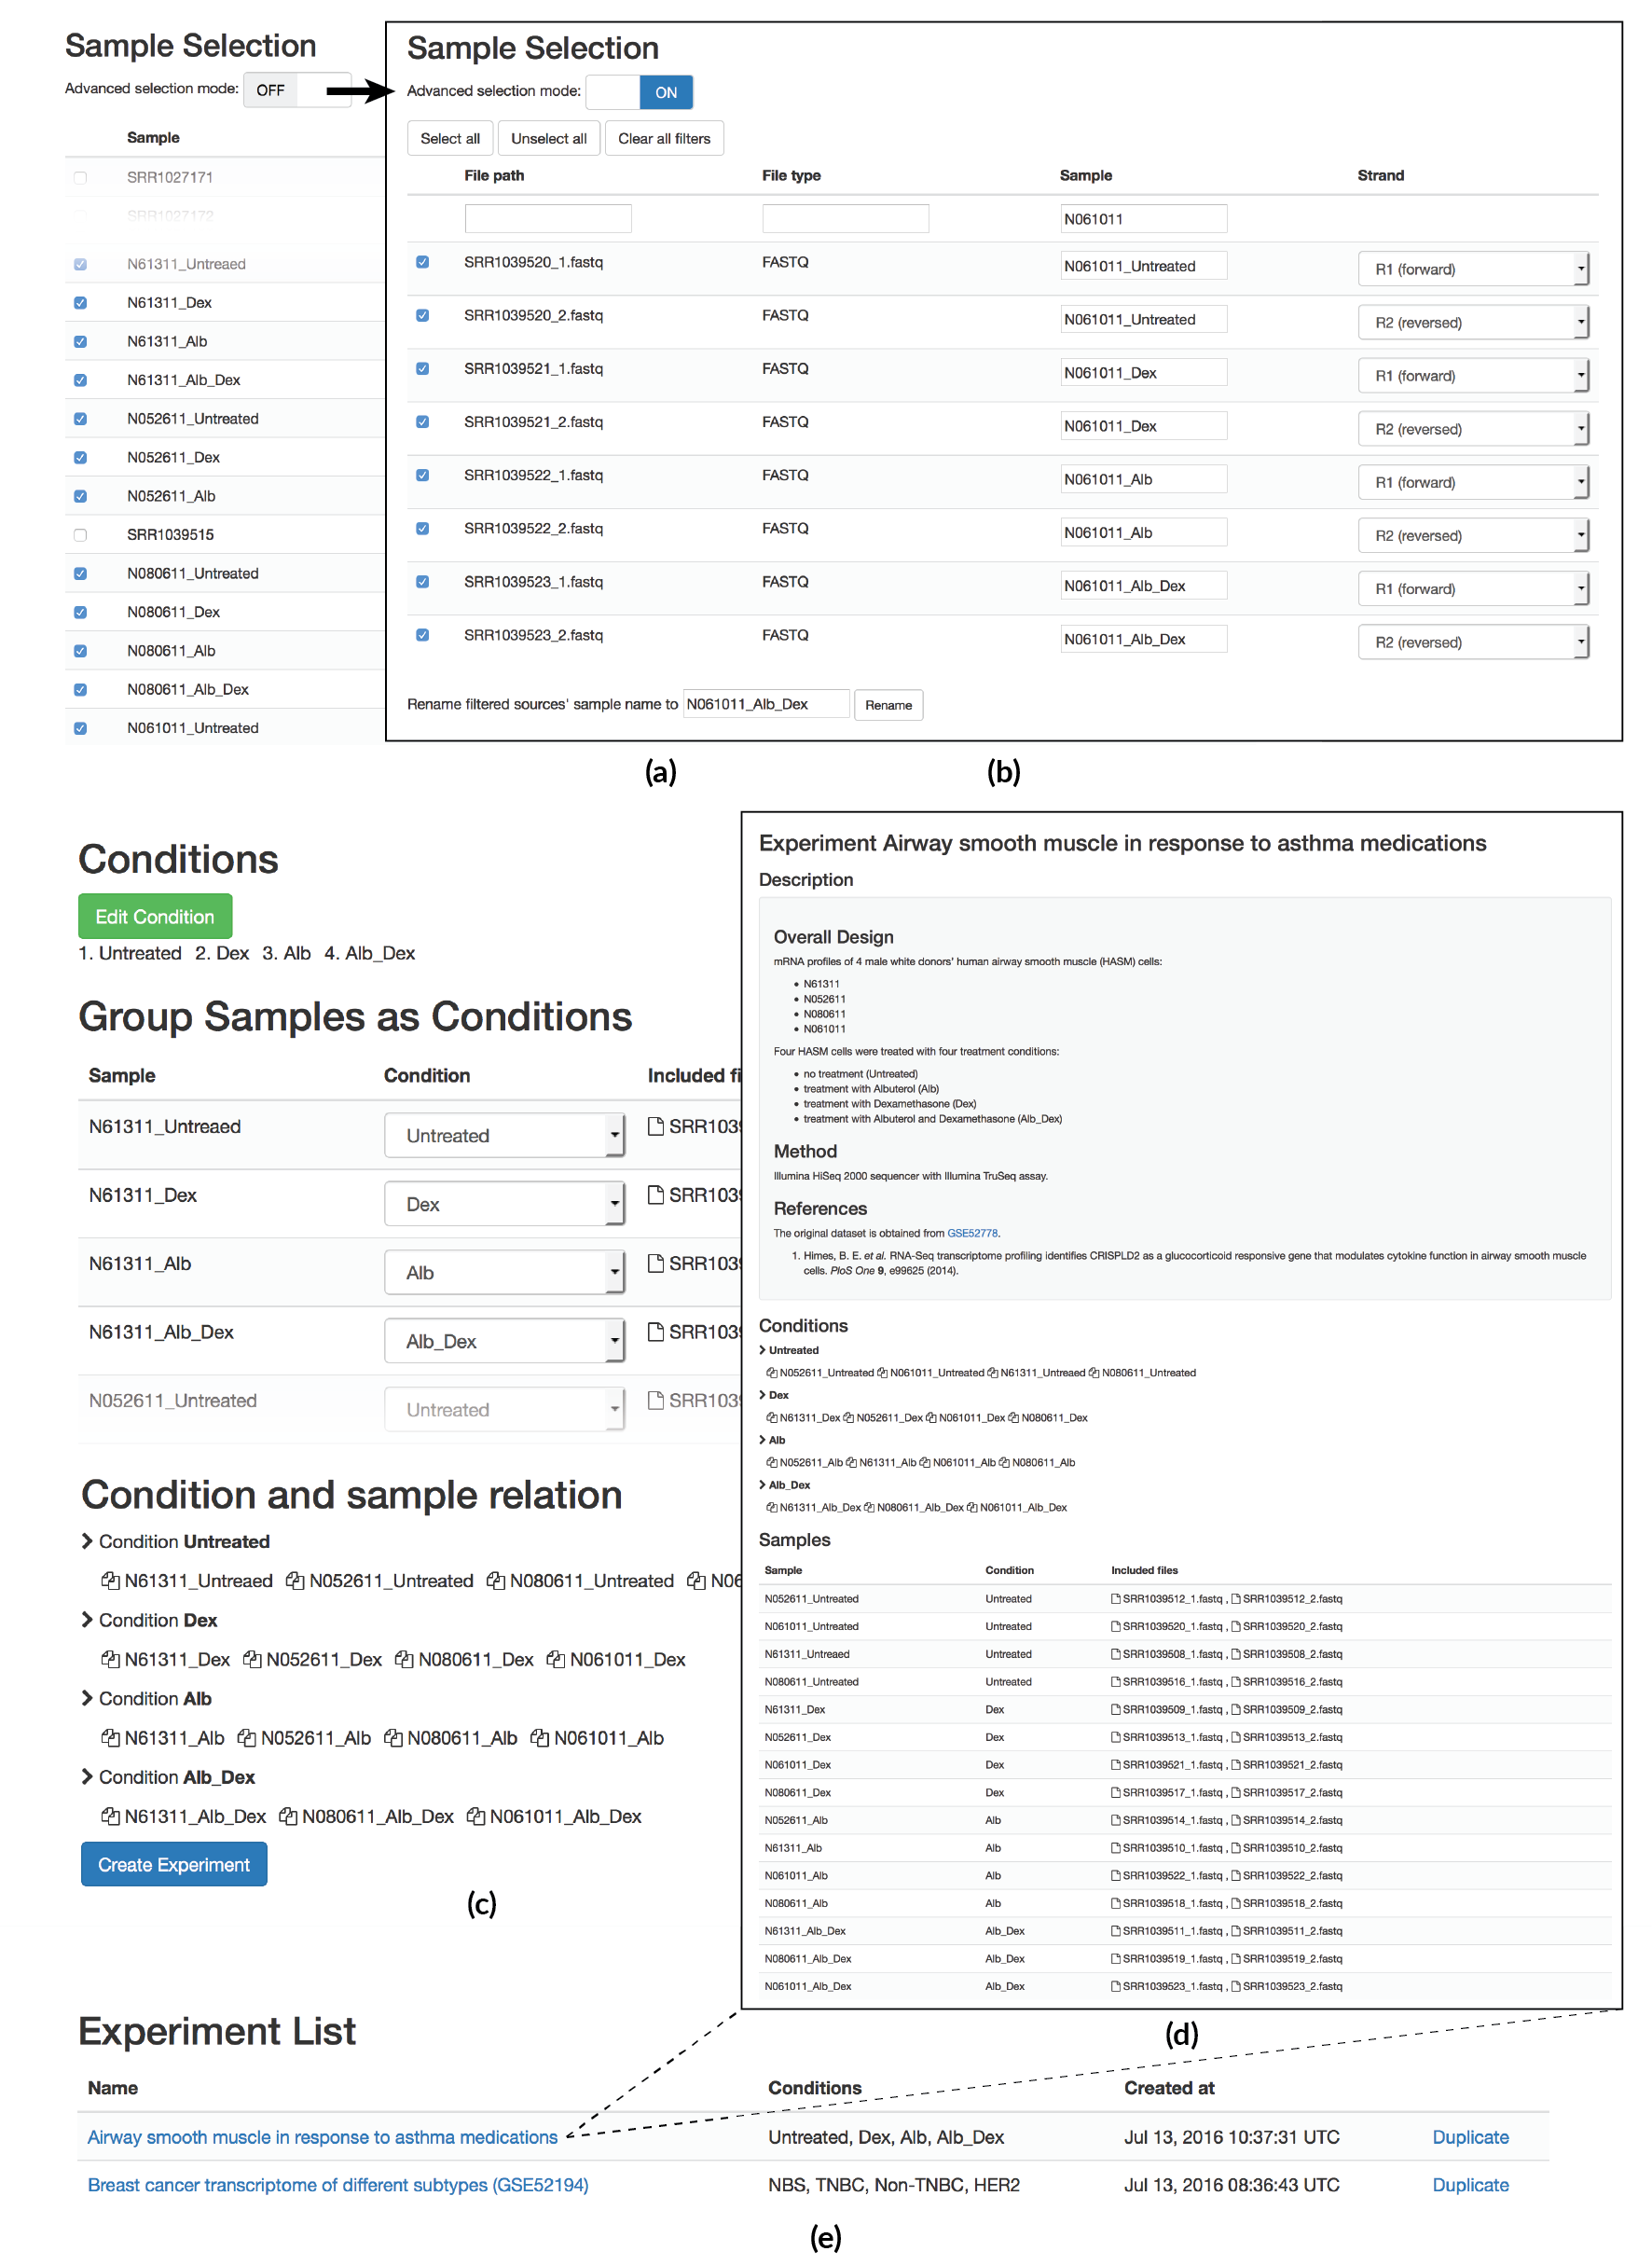
\includegraphics[width=1\textwidth]{images/biocloud_experiment_sample_condition}
\caption[Experiment design on BioCloud (cont'd)]{
    Experiment design on BioCloud (cont'd).
    (a)
    (b)
    (c)
    (d)
    (e)
}
\label{fig:biocloud-experiment-design}
\end{figure}



% general description
Experiment design groups selected samples into user defined conditions to
represent the biological experiment design. BioCloud will warn the user if one
try to create experiment without adding any data source. All experiment related
functions are under the menu item ``Experiment''. Here the demo user added all
datasets mentioned in Section~\ref{s:dataset}. When the user created a new
experiment, one was guided to fill in experiment description, select data
sources, create conditions, assign conditions step by step, as shown in
Figure~\ref{fig:biocloud-experiment-design}. User first filled in the
experiment name and description. Experiment description was written using the
Markdown syntax and an editor based on SimpleMDE was provided, as shown in
Figure~\ref{fig:biocloud-experiment-design}(a). Headings, enumerated lists, and
hyperlinks can be created to help user collect all the related information. The
rendered description can be live previewed in full screen side-by-side mode.

% sample selection
To actually construct the experiment design, user first started with sample
selection, as shown in Figure~\ref{fig:biocloud-experiment-design}(b). By
default the simple mode of selection sample was shown, where data sources of
same sample names were selected together and the default sample name was used.
Selected samples were simultaneously shown in the condition design section
below (Figure~\ref{fig:biocloud-experiment-design}(c)) with the help of
reactive programming. All the elements in the experiment design form shares the
same underlying data structure. Therefore, as a sample was selected, all its
data sources are marked as selected and Vue.js updated all the DOMs that
depended on the selected data sources.

% simple and advanced mode
An advanced mode of selection mode was provided so user can have detail control
on the inclusion of samples, as shown in
Figure~\ref{fig:biocloud-experiment-sample-condition}(b). When it is enabled
data sources were listed one by one and their sample names become modifiable.
User can select one strand of a pair-end sample, or override the existed sample
name of data sources. Data sources can be filtered based on file name, file
type, and sample name.

% condition
By default samples are of condition ``(All)'', a special condition implying the
sample does not belong to any given condition. Currently no pipeline requires
the special condition but it is implemented so custom pipeline can let user
specify experiment-wise input. By default there were two conditions: Control
and Testing. User can remove, edit, and add conditions, as shown in
Figure~\ref{fig:biocloud-experiment-design}(d). They were dynamically rendered
as available options of selected sample's conditions, as shown in
Figure~\ref{fig:biocloud-experiment-design}(e). Note that it is considered safe
and there will be no data loss if user later modifies the condition name.
Order of conditions was kept in the database. In analysis, condition specified
later was compared with those specified earlier for each condition pair.
Generally, one should put control or normal condition as the first condition.
In the figure, breast cancer dataset defined conditions: NBS, TNBC, Non-TNBC,
HER2 in order, where NBS was the normal condition of the dataset. As user was
designing the conditions, a preview of the current experiment was displayed in
the last section, as shown in
Figure~\ref{fig:biocloud-experiment-sample-condition}(c).

%experiment list
User can view one's submitted experiments at the experiment list view, as shown
in Figure~\ref{fig:biocloud-experiment-sample-condition}(e). Detail of the
experiment can be found by clicking the link of each experiment in the
experiment list view, as shown in
Figure~\ref{fig:biocloud-experiment-sample-condition}(d). Users are not allowed
to modify the experiment conditions, otherwise existed analyses would have
uncertain experiment design. However, one can build a new experiment based on a
existed experiment design.



\section{Analysis design}

\begin{figure}[!p]
\centering
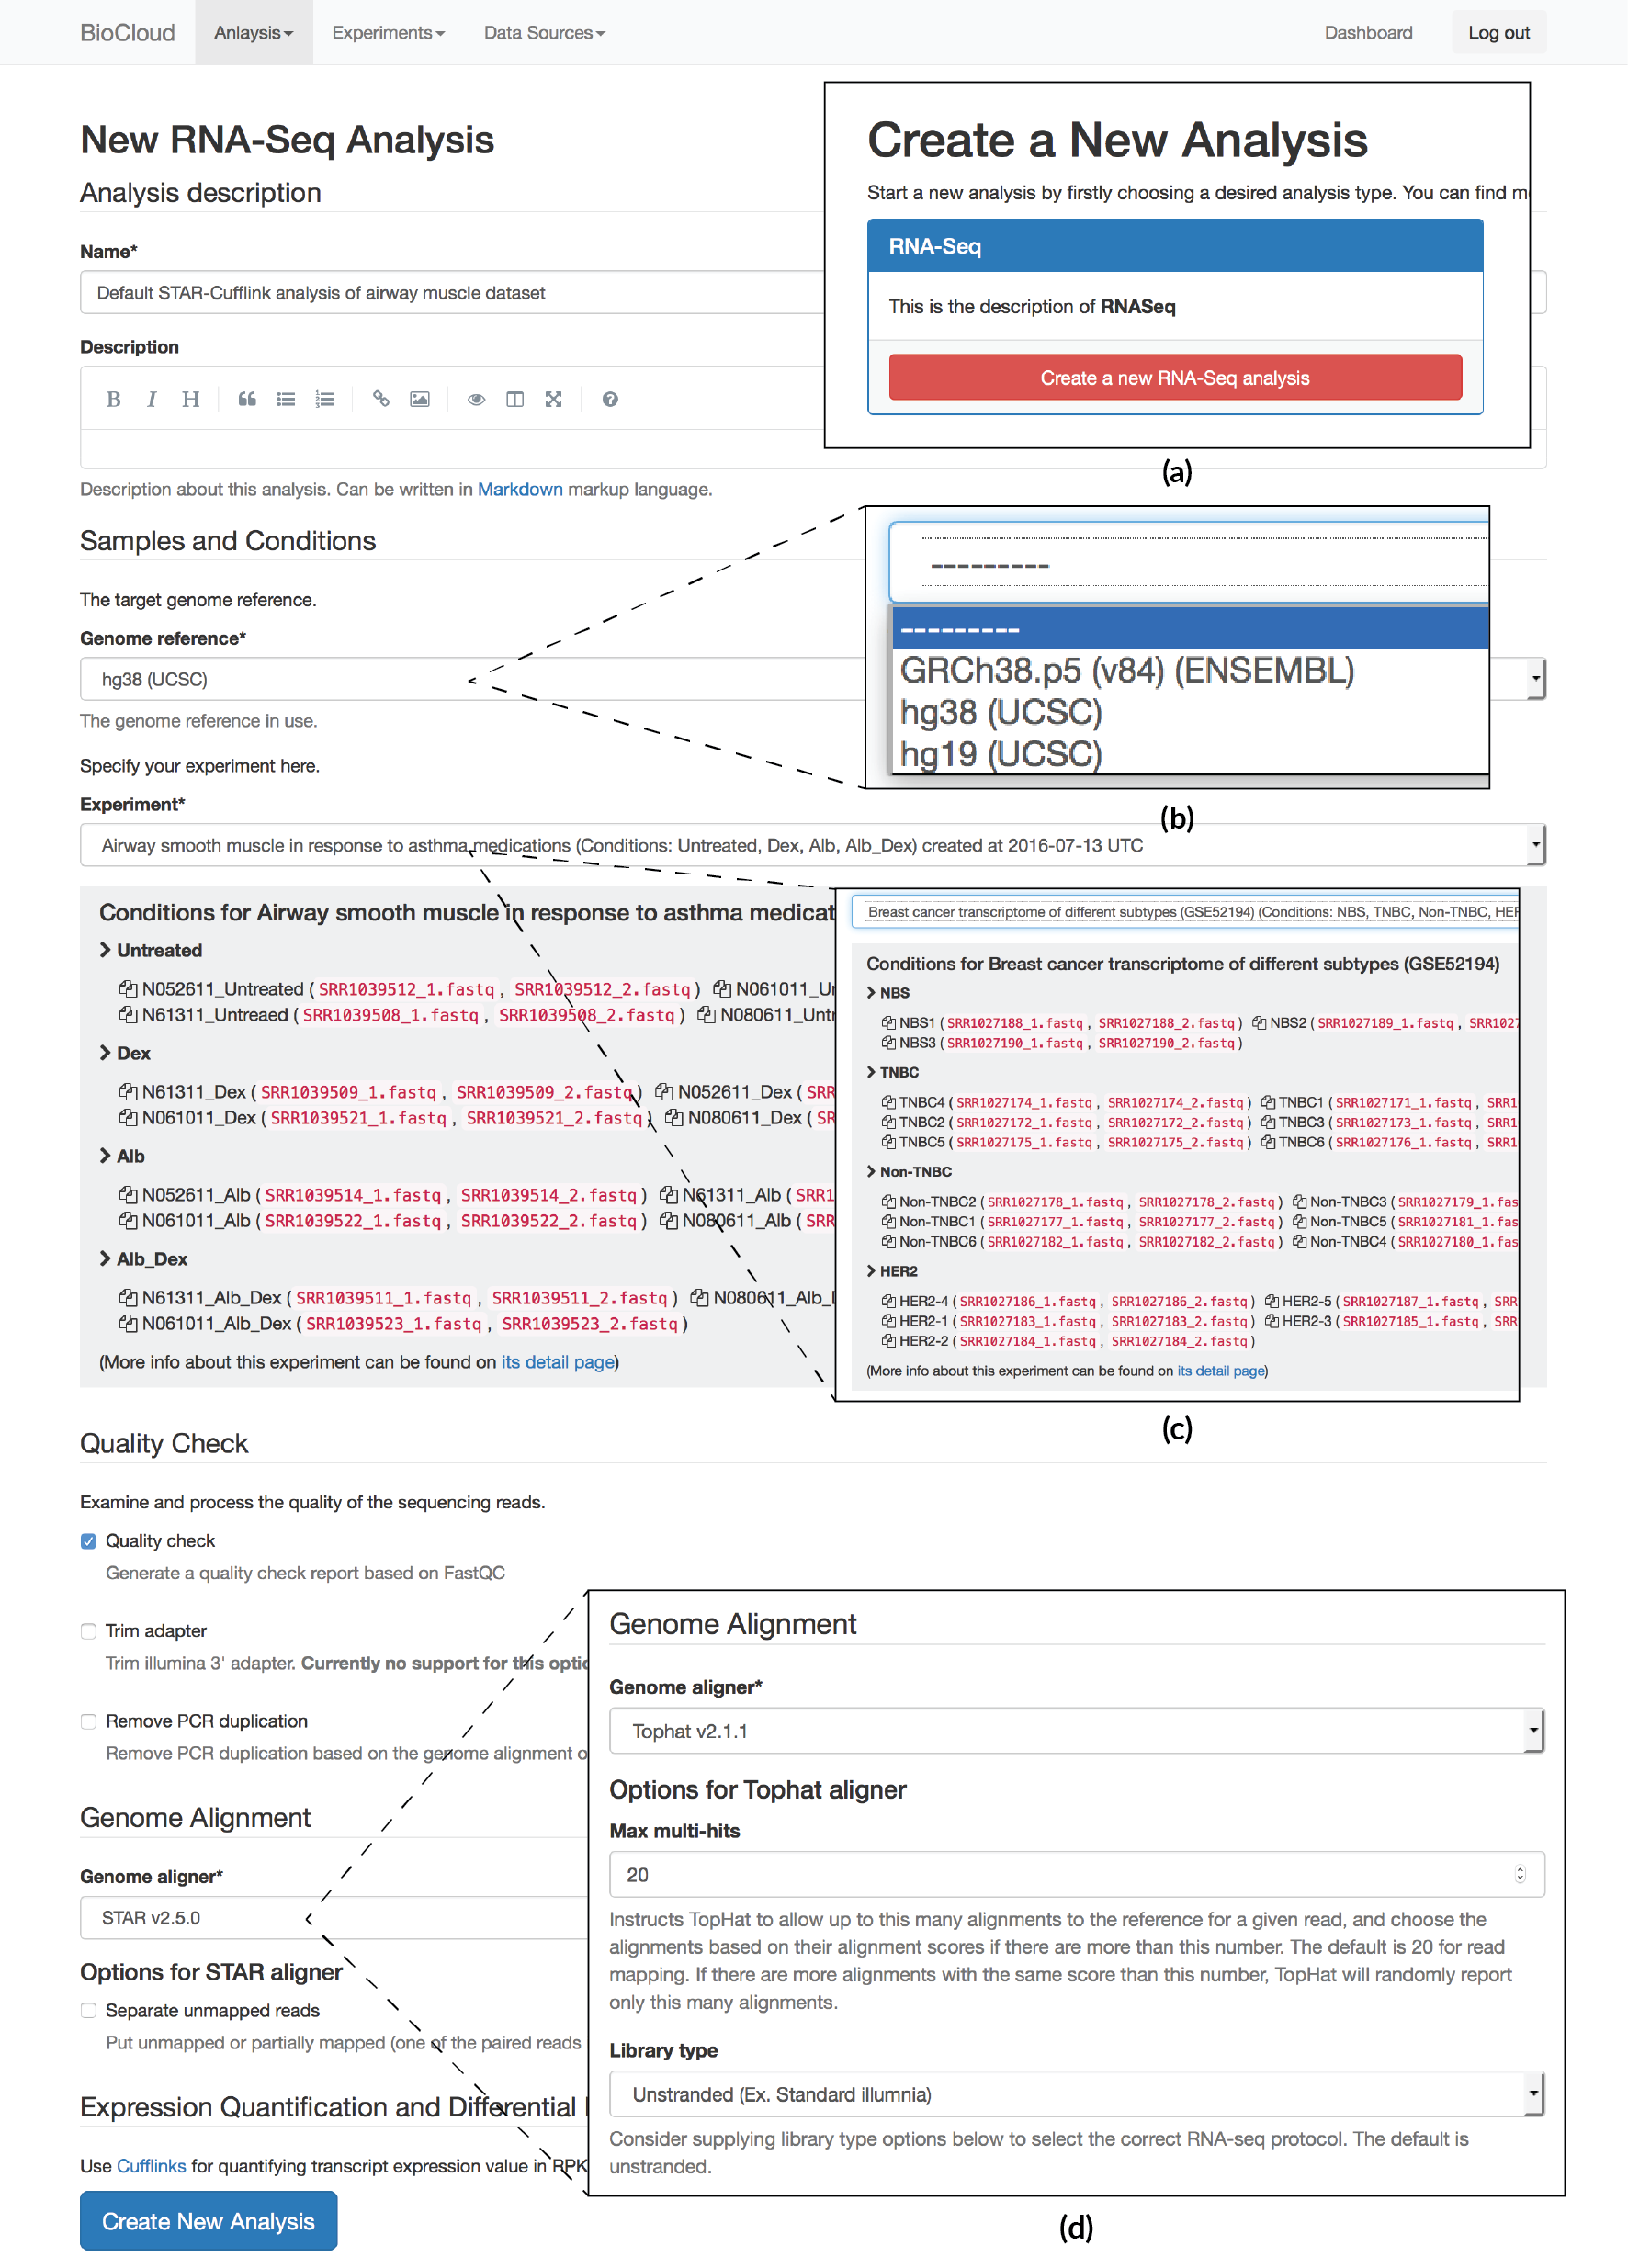
\includegraphics[width=1\textwidth]{images/biocloud_analysis_design}
\caption[Analysis design on BioCloud]{
    Analysis design on BioCloud.
}
\label{fig:biocloud-analysis-design}
\end{figure}



Analysis binds an experiment design and executes one of the available pipelines
with given genome reference and parameters. First user chose the pipeline to
execute, as shown in Figure~\ref{fig:biocloud-analysis-design}(a). It was a
portal which gathered all currently available pipelines defined in the BioCloud
source code. In Figure~\ref{fig:biocloud-analysis-design}, the demo user
selected the Cufflink-based RNA-Seq pipeline. User was then guided to a new
dedicated page for the selected analysis design form. Similar to experiment
design, user can specify name and description in Markdown syntax for the
new analysis.

Some parts of the analysis design form were the same for all analysis
pipelines. All analysis pipelines requires genome reference and experiment
design as input. Available genome references were defined by staff or superuser
via the BioCloud admin interface, whose name and provider combined as the
option name as shown in Figure~\ref{fig:biocloud-analysis-design}(b). Here the
human genome reference hg38 provided by UCSC was chosen. User continued to
select the experiment design in use. User can select by the name of one's own
experiment designs, whose conditions and samples will be dynamically rendered
once user made a choice, as shown in
Figure~\ref{fig:biocloud-analysis-design}(c). A link to the experiment detail
view was also provided for more information. Here the human airway smooth
muscle dataset was used.

Finally, rest of the analysis design form was specially defined for
Cufflink-based RNA-Seq pipeline. As described in
Section~\ref{s:rnaseq-pipeline}, there are three available genome aligners in
this pipeline. Each of the aligner has different option sets. Therefore, as
user selected one aligner, only the corresponding options were shown. In
Figure~\ref{fig:biocloud-analysis-design}(d), as user changed the aligner from
STAR to Tophat2, different options were displayed.



\section{Job queue monitoring}

% email notification
Figure~\ref{fig:biocloud-job-monitor}.

\begin{figure}[!p]
\centering
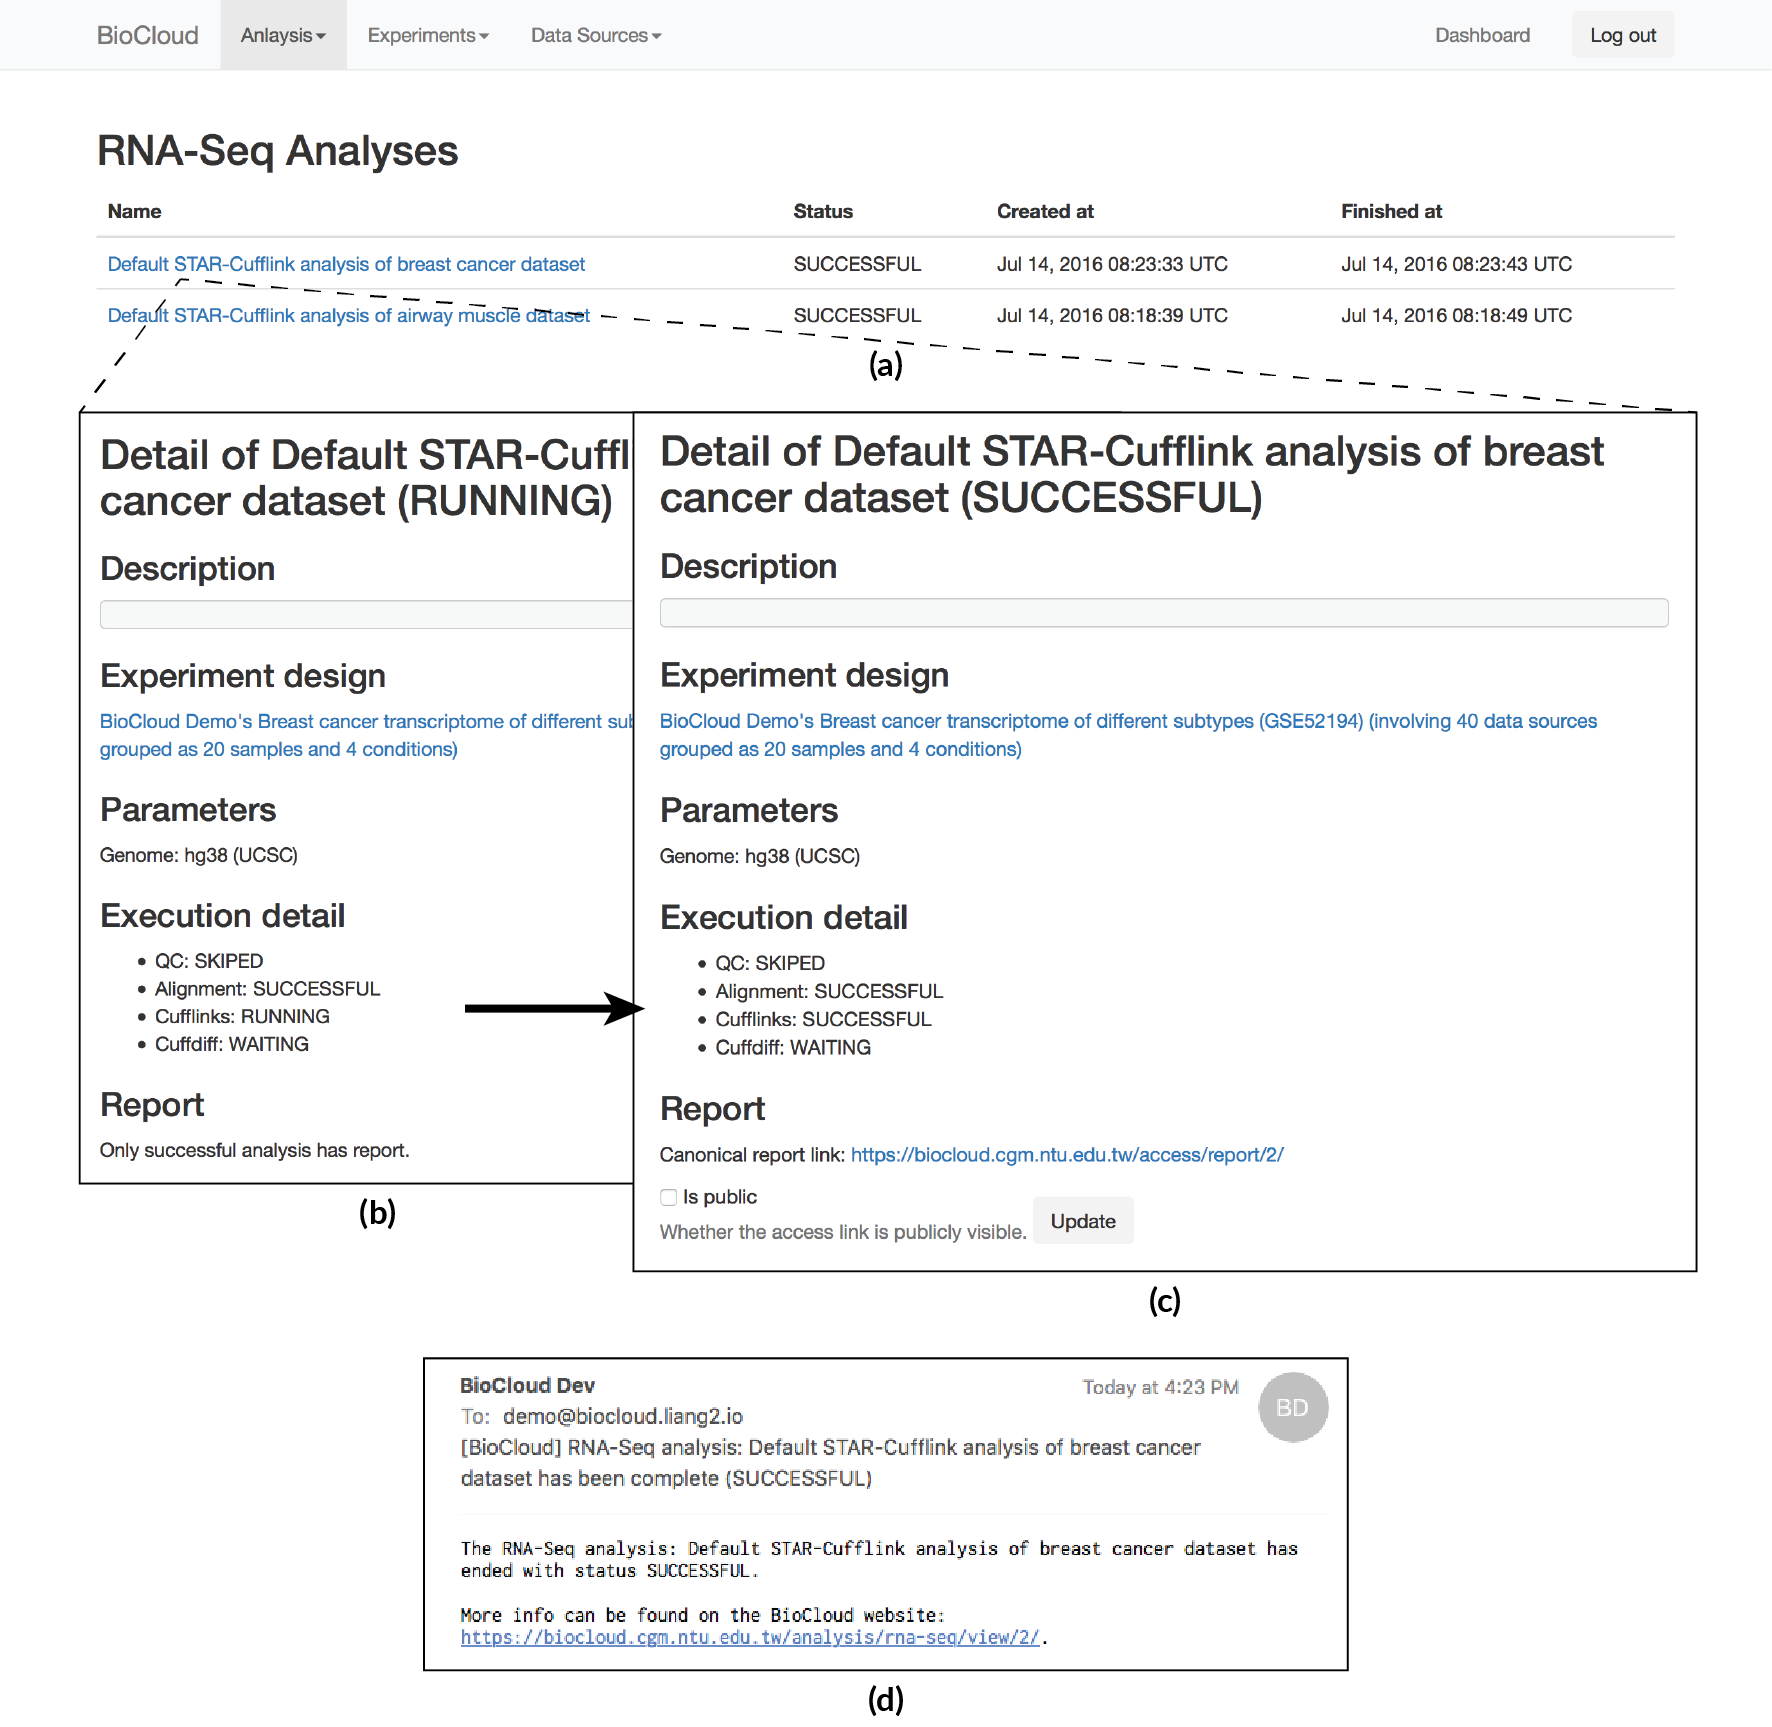
\includegraphics[width=1\textwidth]{images/biocloud_job_monitor}
\caption[Job monitoring on BioCloud]{
    Job monitoring on BioCloud.
}
\label{fig:biocloud-job-monitor}
\end{figure}




\section{Admin}
\label{s:biocloud-admin}

Figure~\ref{fig:biocloud-admin}.

\begin{figure}[!p]
\centering
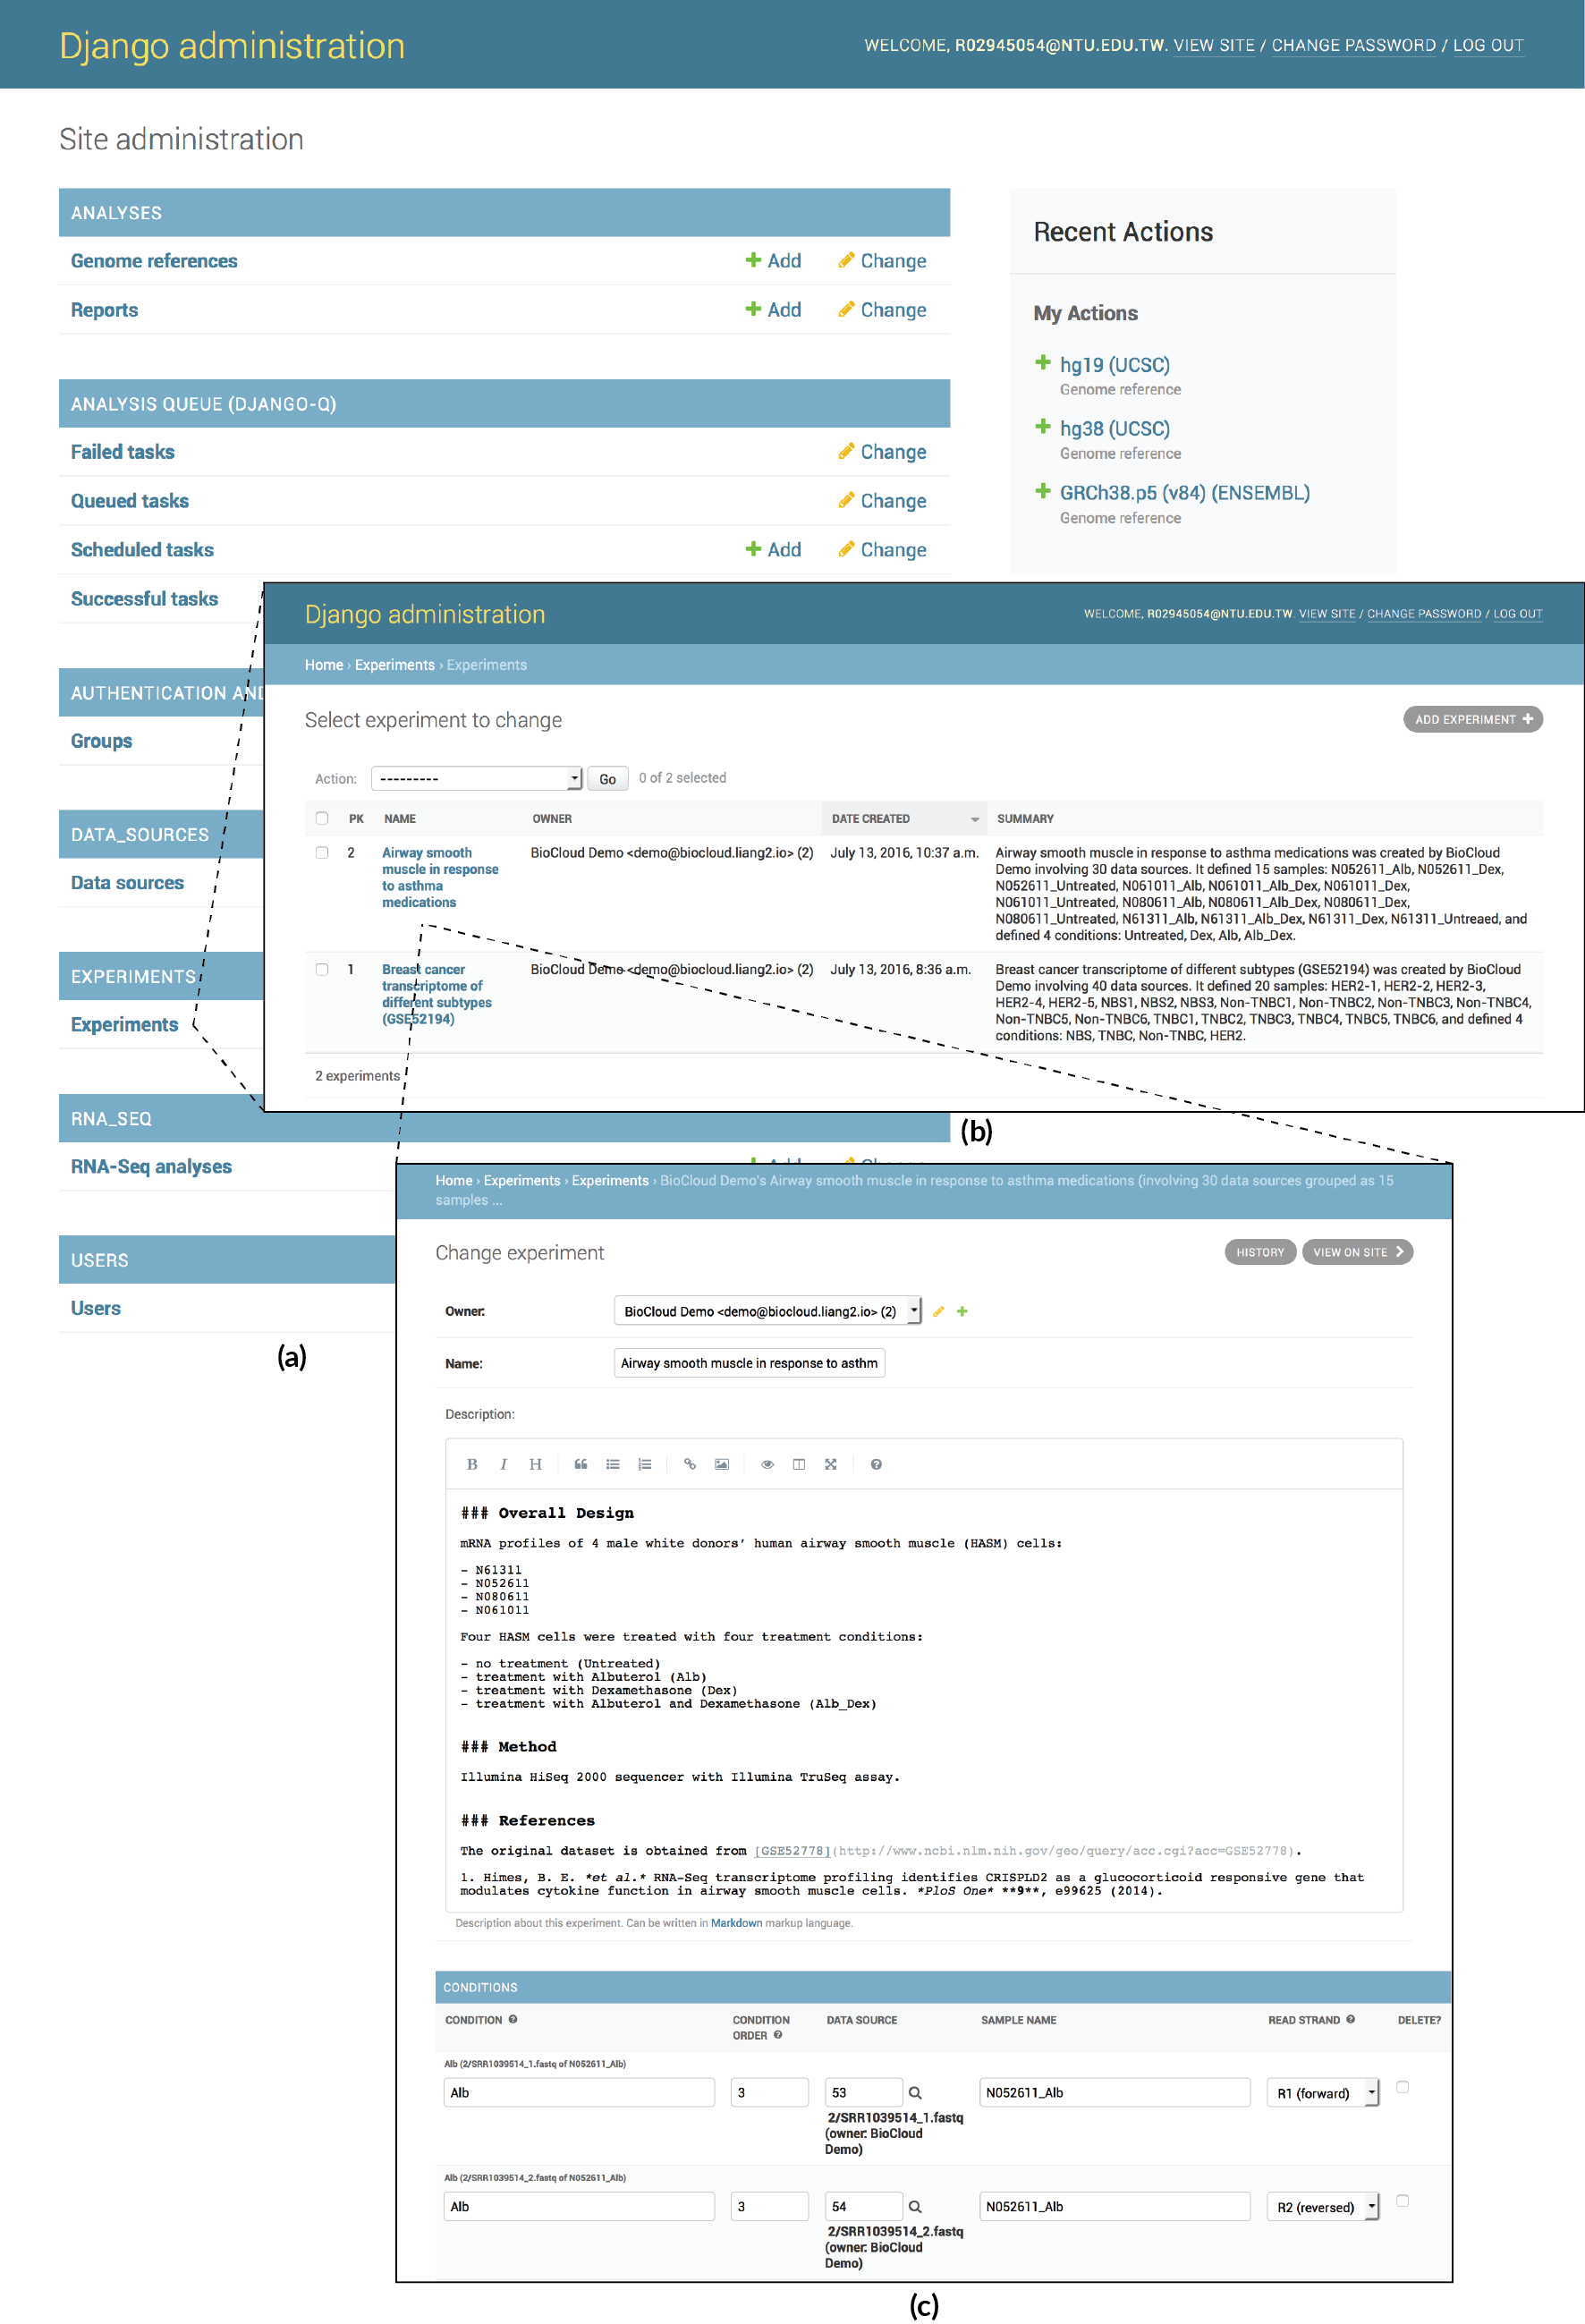
\includegraphics[width=1\textwidth]{images/biocloud_admin}
\caption[Admin interface of BioCloud]{
    Admin interface of BioCloud.
}
\label{fig:biocloud-admin}
\end{figure}






\section{Result summary report}


\subsection{Report and result access}
\label{s:report-result-access}

Figure~\ref{fig:report}.
\begin{figure}[!tb]
\centering
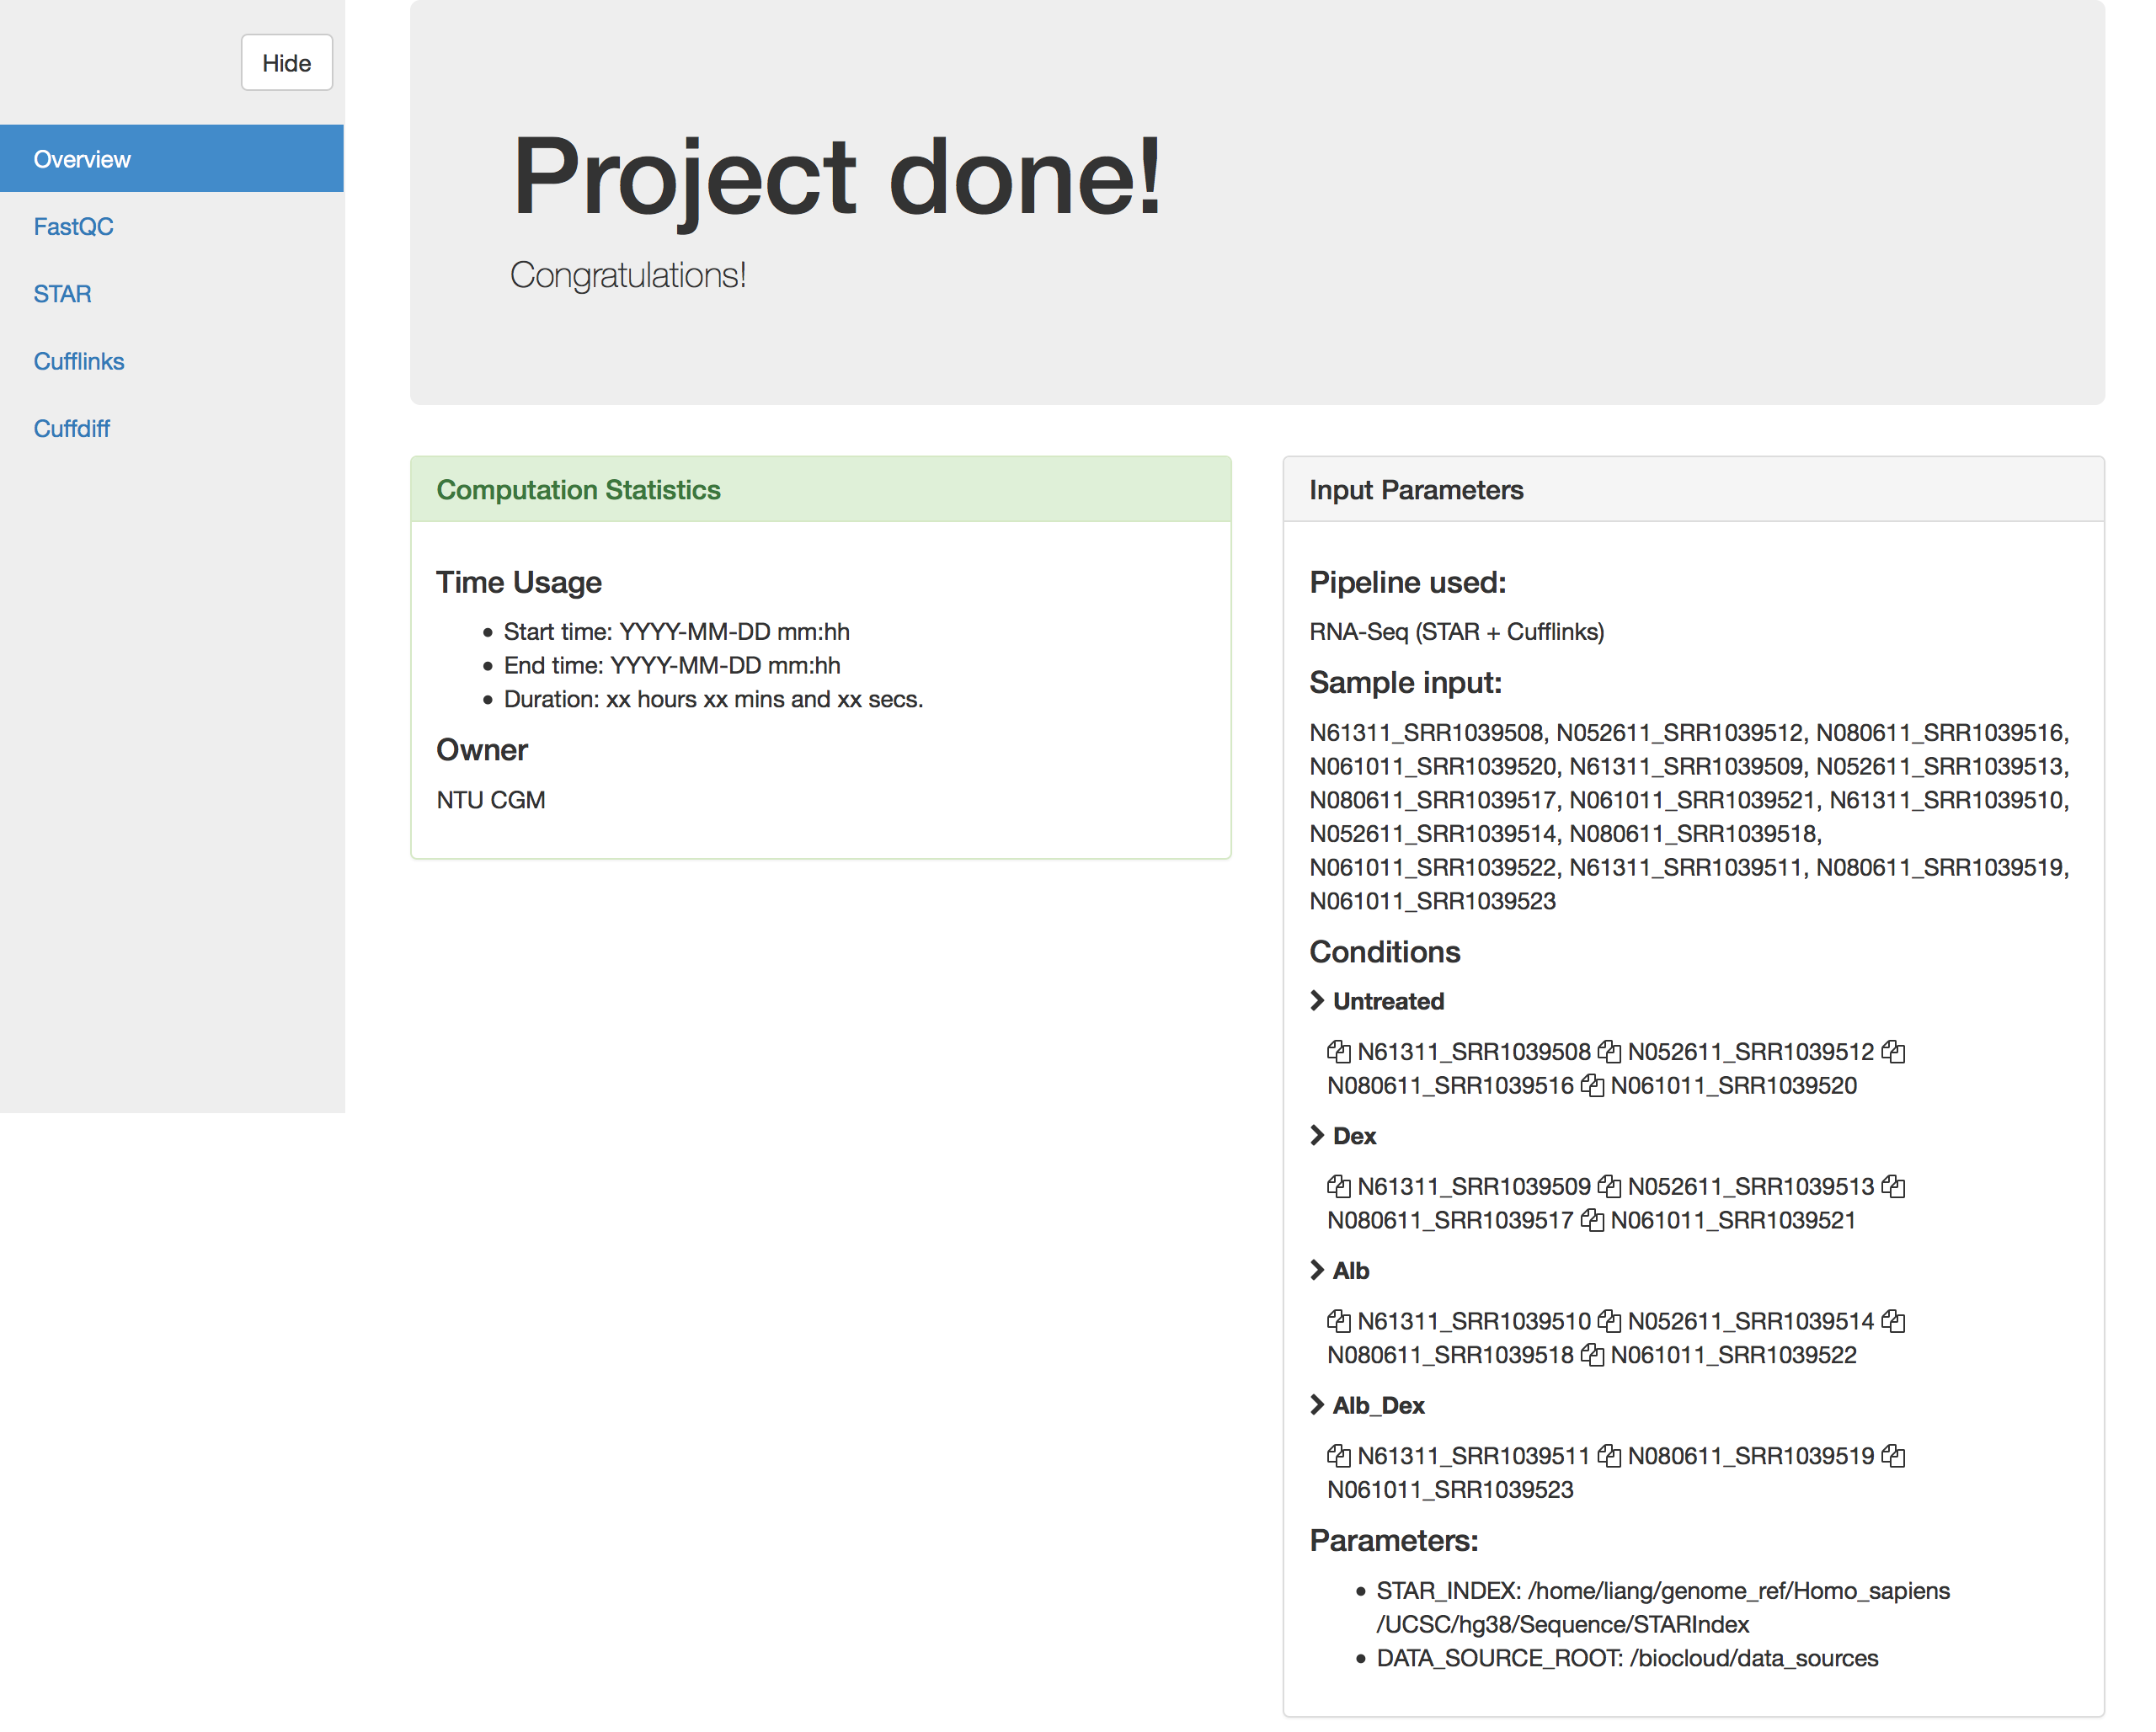
\includegraphics[width=1\textwidth]{images/report_home}
\caption[Result summary report]{
    Result summary report.
}
\label{fig:report}
\end{figure}





\subsection{Integration with public genome browser}

\begin{CVerbatim}[fontsize=\small]
track type=bam name="NBS1"
bigDataUrl=https://biocloud.cgm.ntu.edu.tw/access/<auth key>/result/
STAR/NBS1/Aligned.sortedByCoord.out.bam
\end{CVerbatim}

Figure~\ref{fig:result-genome-browser}.
\begin{figure}[!p]
    \centering
    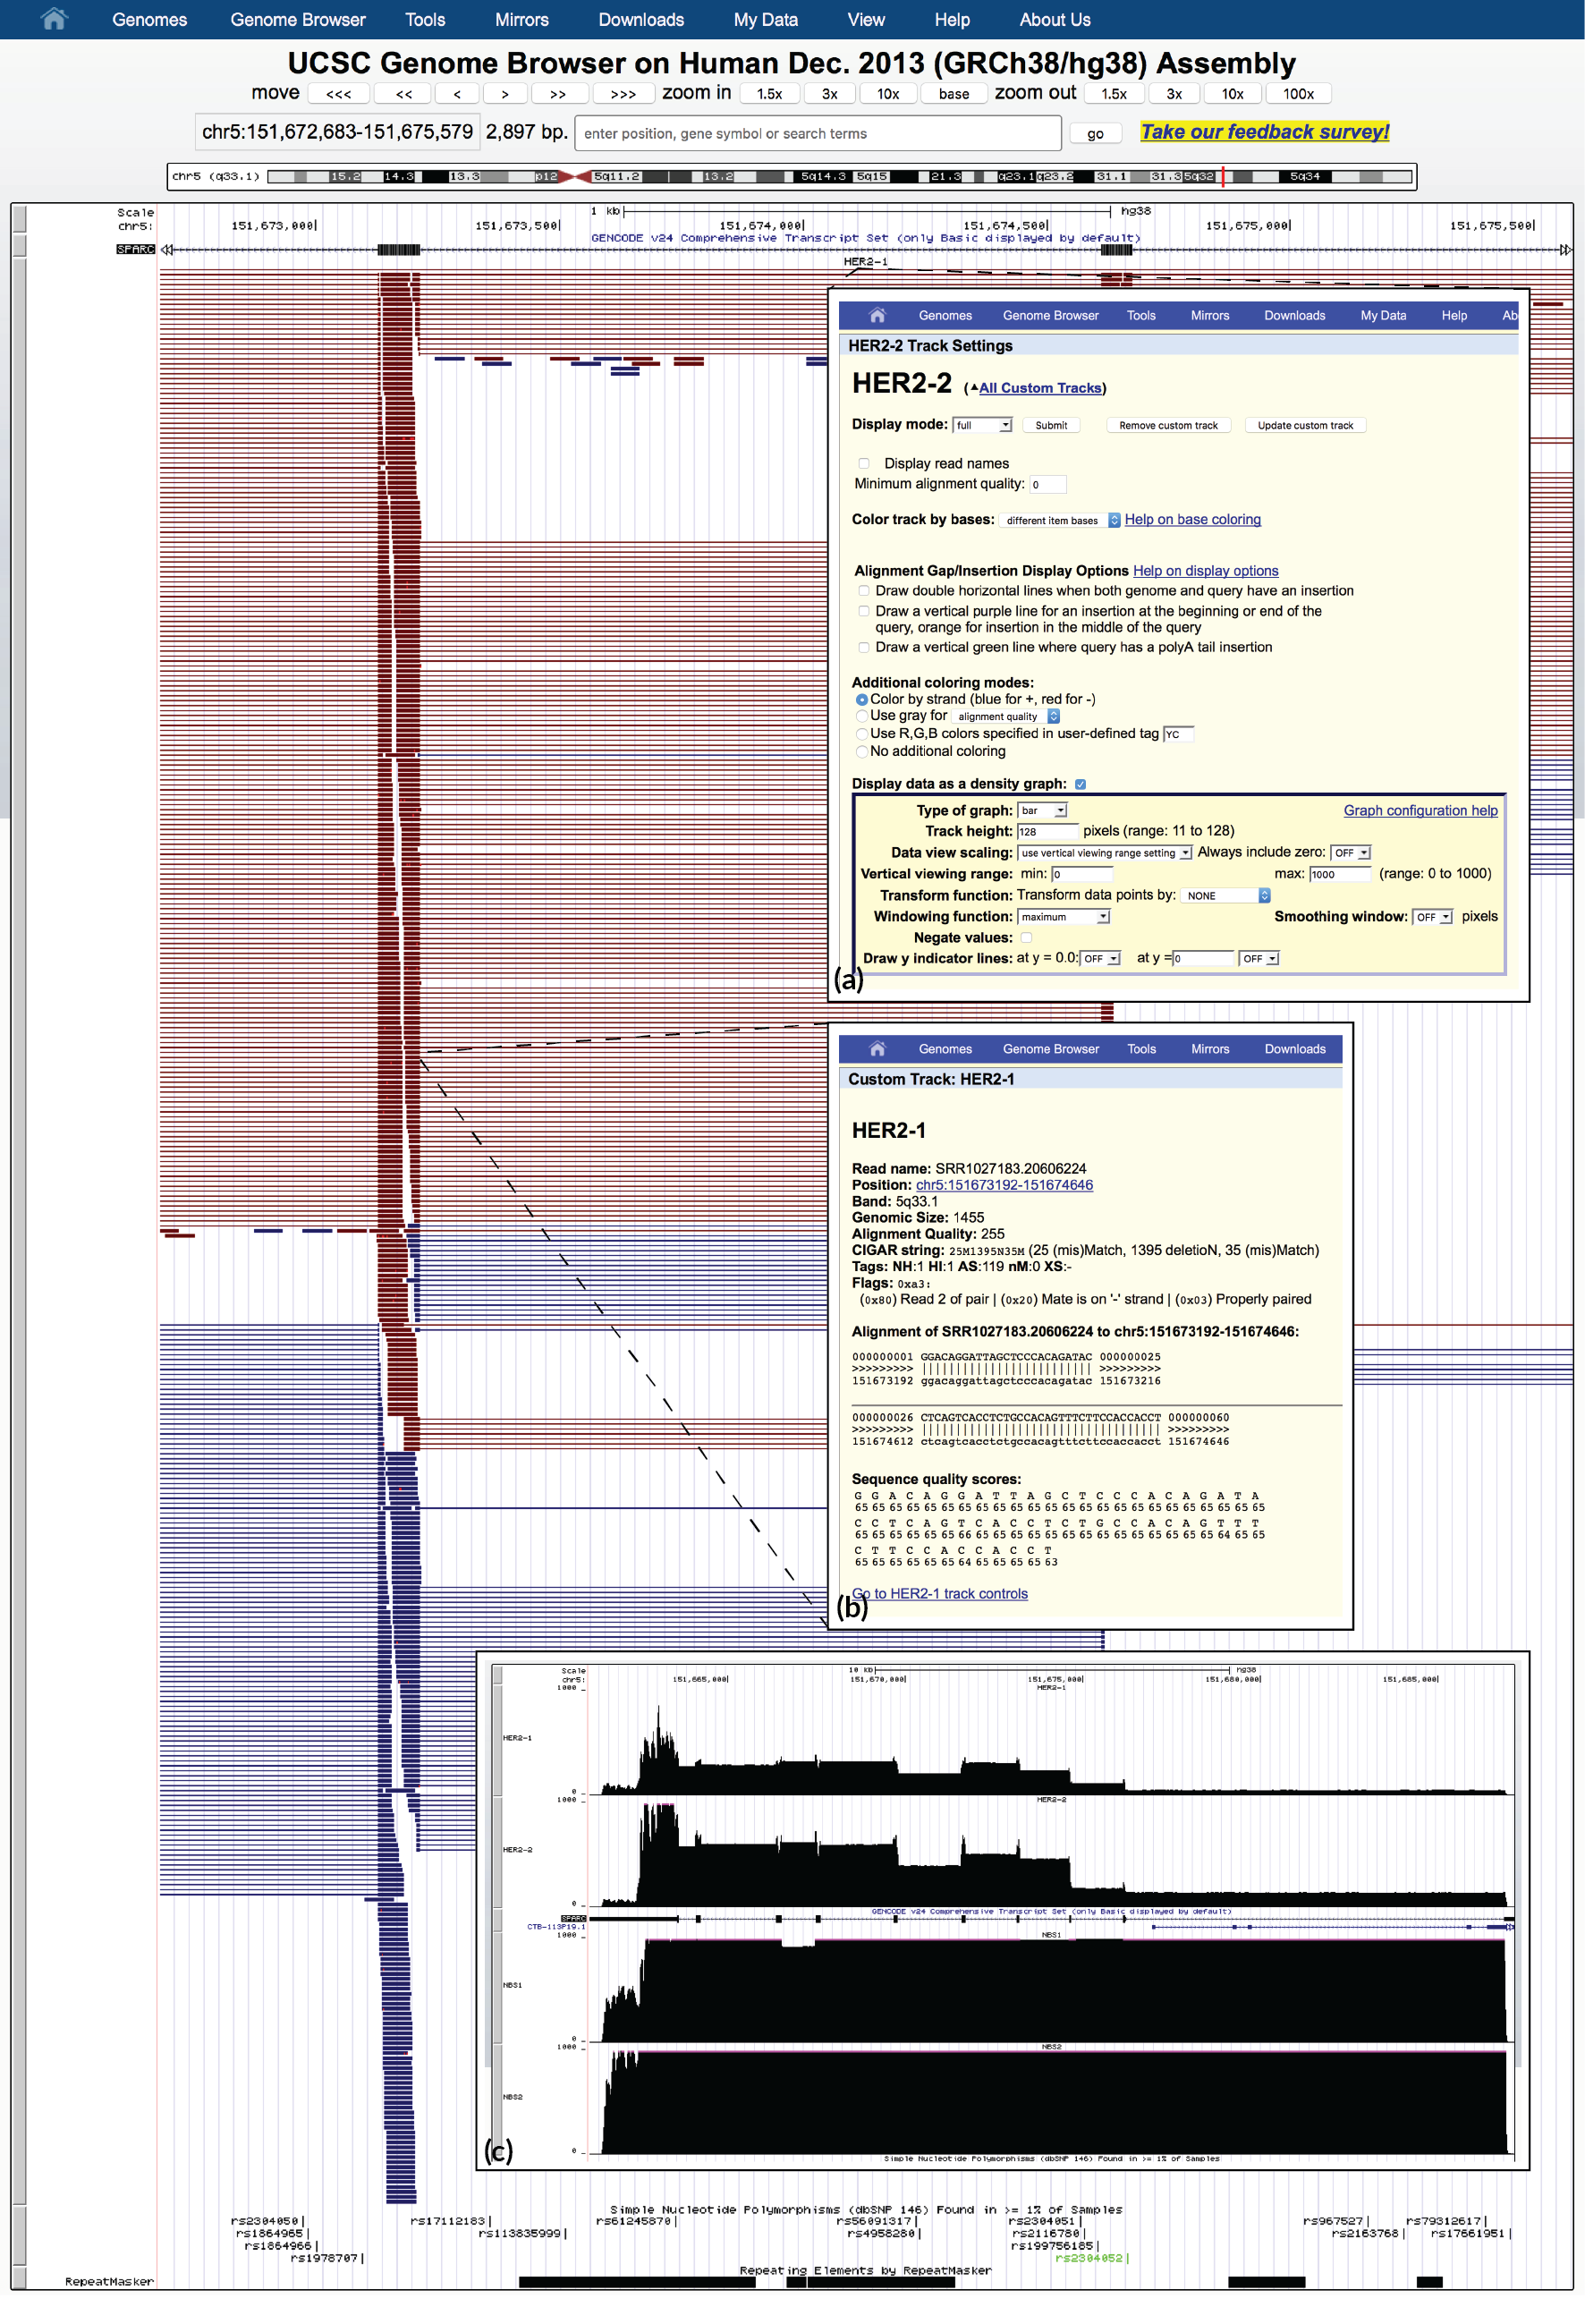
\includegraphics[width=1\textwidth]{images/result_genome_browser}
    \caption[Result integration with genome browser]{
        Result integration with USCS genome browser. Alignment of HER2-1 sample
        was shown. Display options can be tuned in the panel shown in (a). By
        clicking on an read, detail alignment information poped up as shown in
        (b). In (c), genome browser was configured to display the coverage
        depth of four samples simultaneously.
    }
    \label{fig:result-genome-browser}
\end{figure}




\subsection{QC}

Figure~\ref{fig:report-qc}.
\begin{figure}[!tb]
\centering
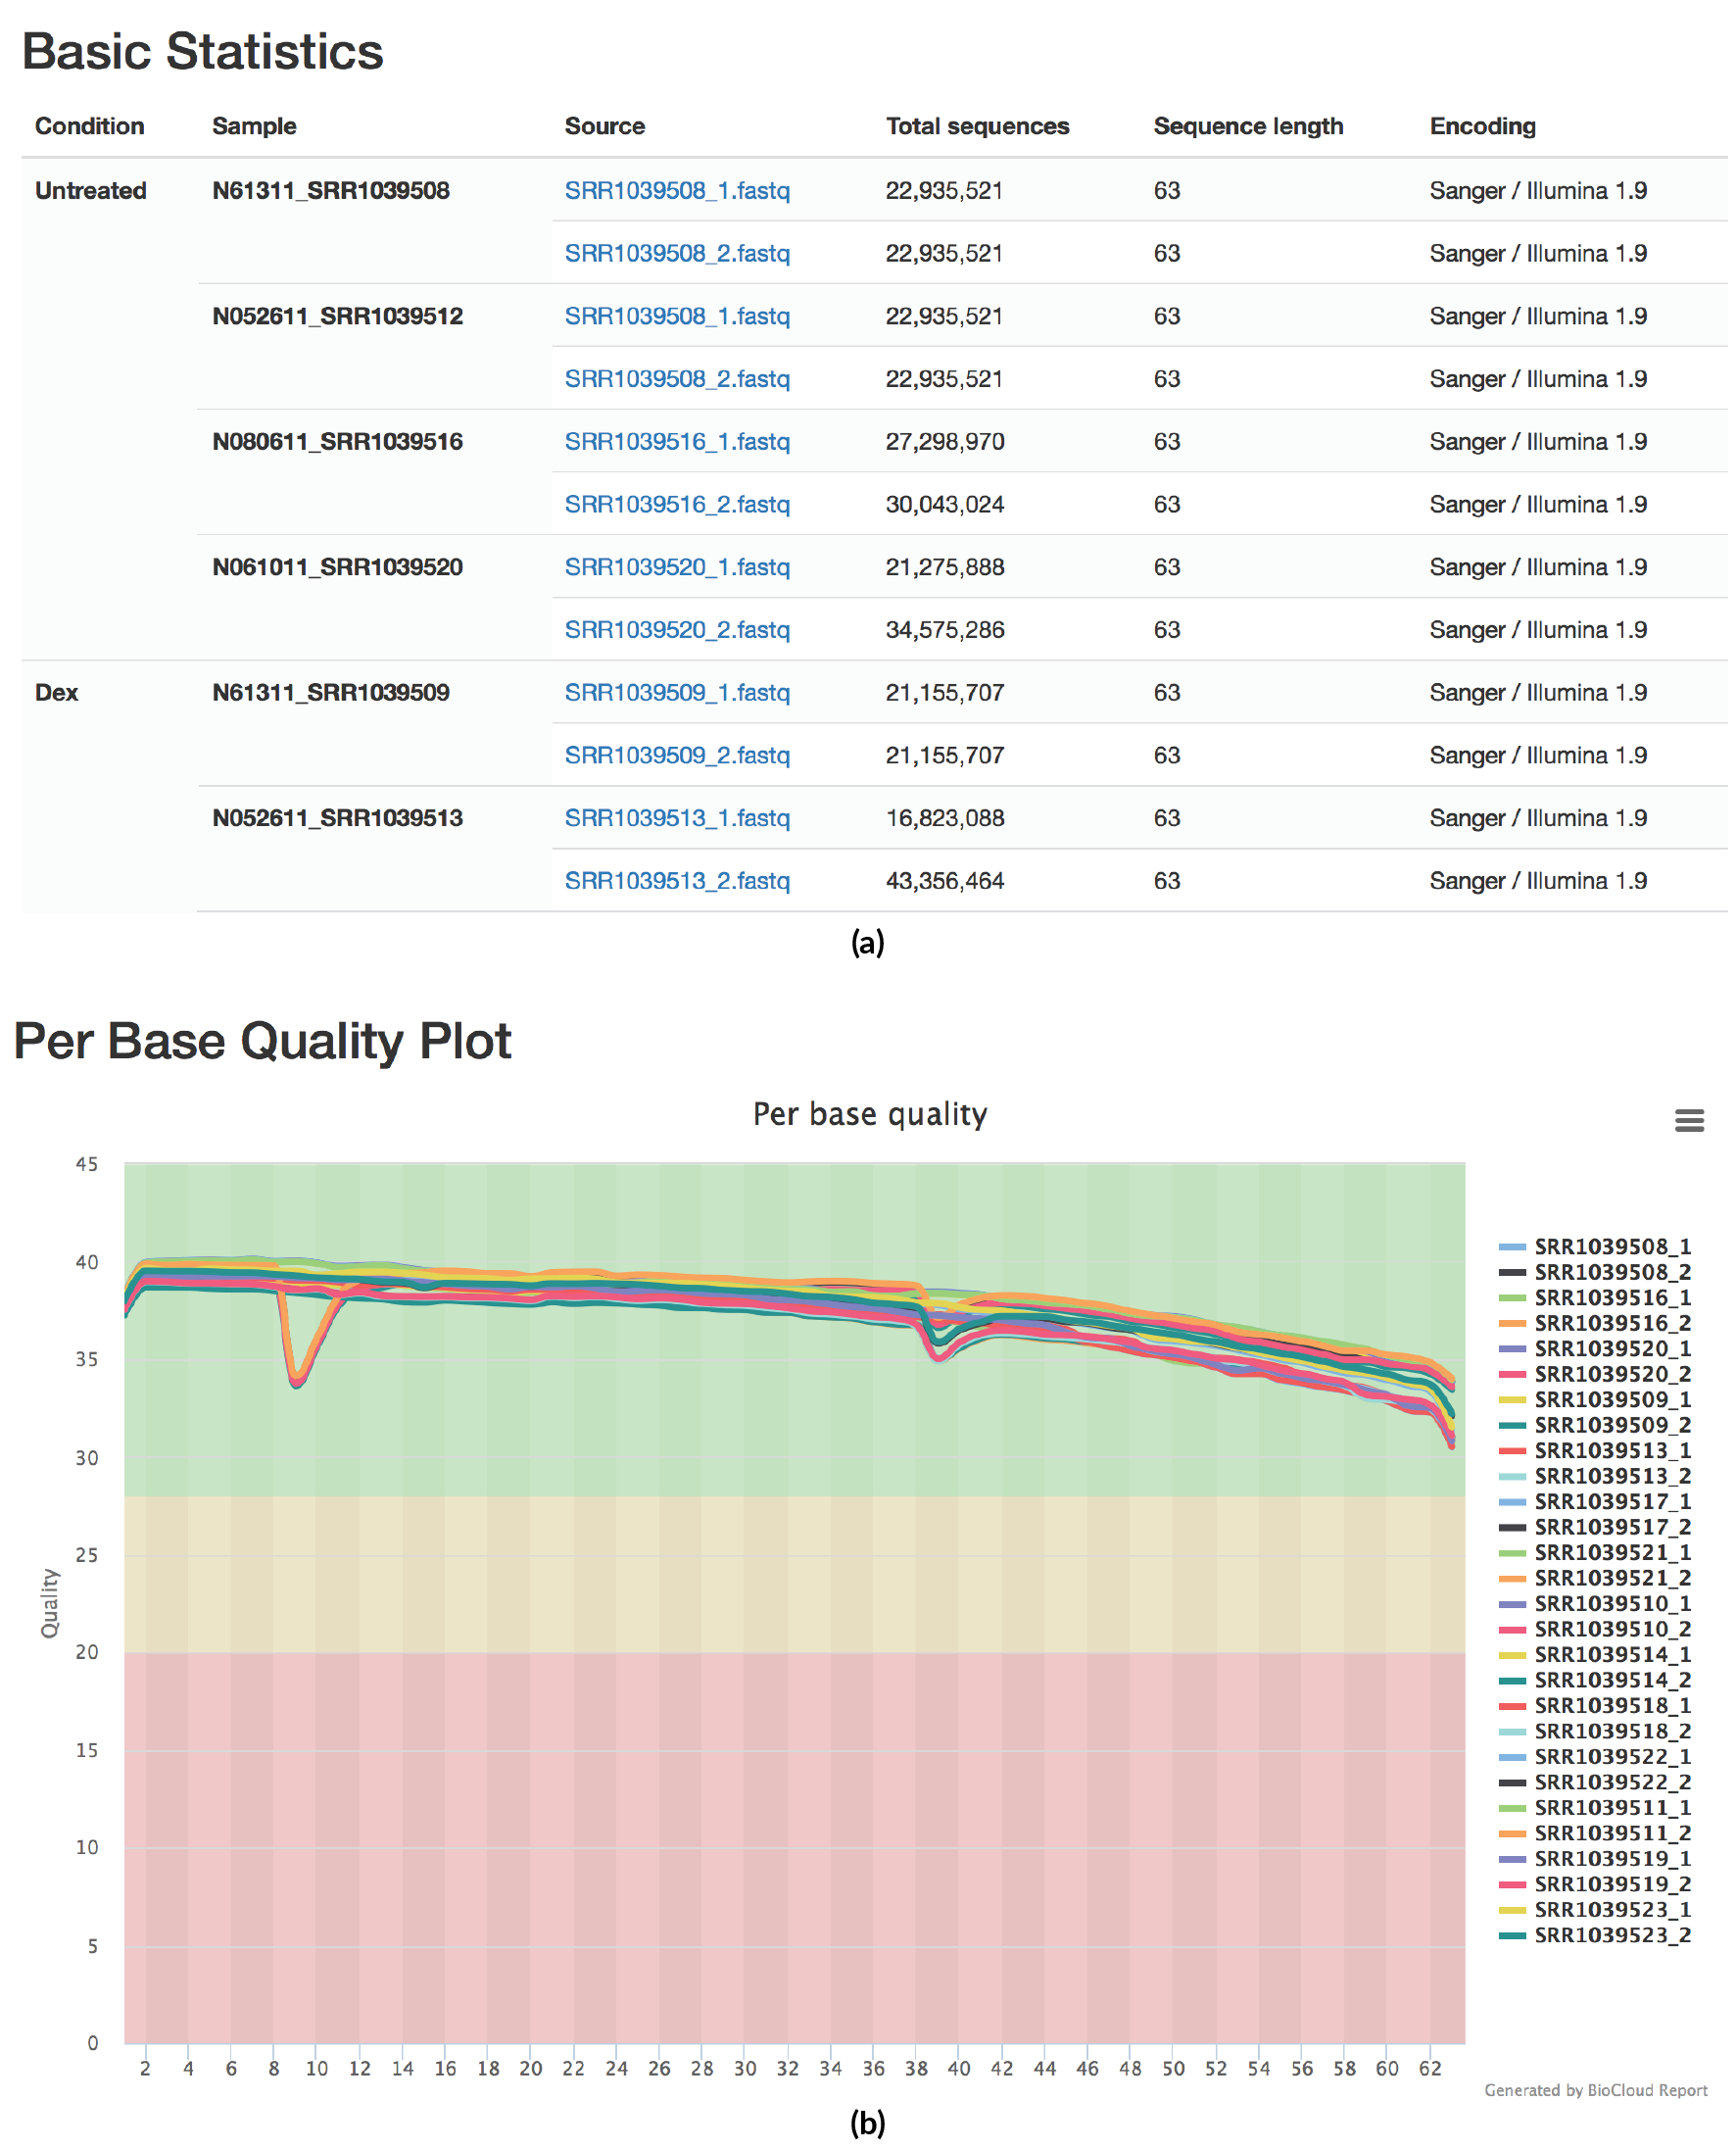
\includegraphics[width=1\textwidth]{images/report_qc}
\caption[Quality check page of report]{
    Quality check page of report.
}
\label{fig:report-qc}
\end{figure}


% \subsection{Alignment - STAR}
% \subsection{Cufflinks}
% \subsection{DESeq2}

% vim: set textwidth=79 spell:
